\section{Overview}
In this section we will provide a high-level view and description of the components that our system is made of. The architecture chosen for our system is a three-tier one. The major advantages of this architectural style is the decoupling of the application logic from the presentation logic and the data persistence concerns. Further details about the characteristics of this architectural style will be given in section 2.6, for now we will proceed with the general overview of the system. In the picture below is illustrated a high-level view of the system with an informal notation, where each rectangular box represents a high-level computational unit of the system, meanwhile the double-edged arrow represents 
 the interaction between two components. \\
\begin{figure}[H]
    \centering
    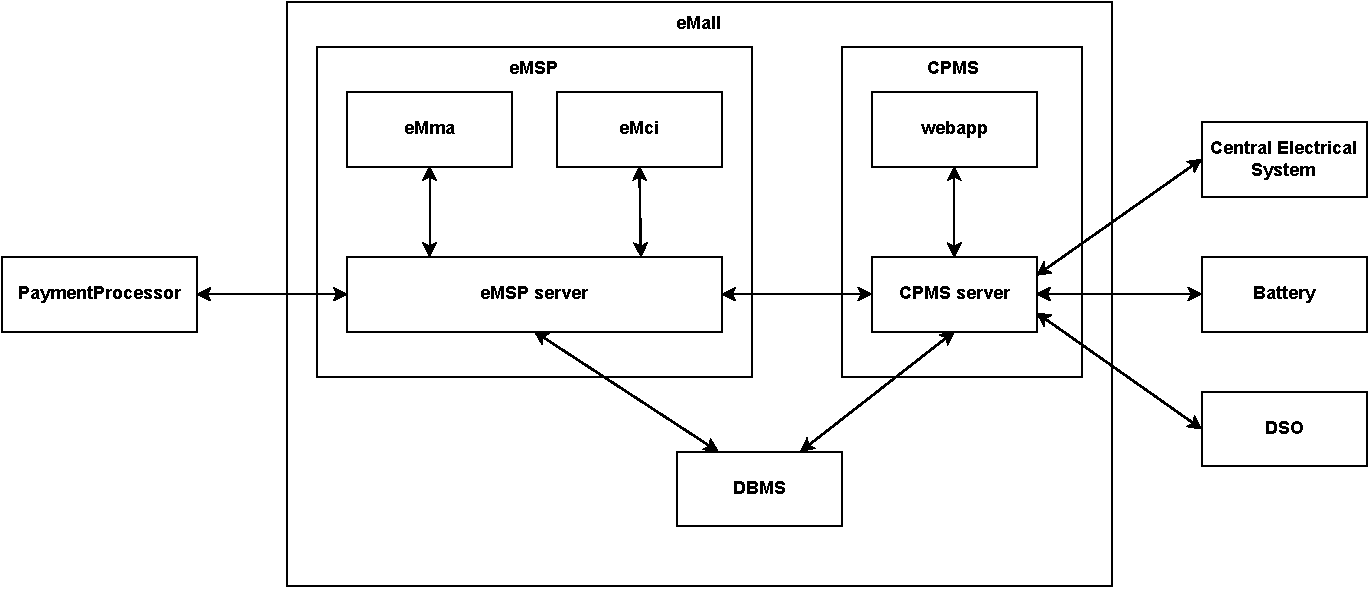
\includegraphics[width=0.8\textwidth]{Images/cp2/overview.pdf}
    \caption{High level description of the components and their interactions}
\end{figure}

\par
The eMall system, illustrated in the figure, is the objective of this design document. It is clear that the system is divided in two main sub-systems: eMSP and CPMS. This choice is driven by an interoperability requirement of the eMSP and the CPMS with different CPMS and eMSP systems respectively, offered by other companies. Nonetheless, this low-coupling of the CPMS with the eMSP doesn't preclude us from reusing components that have the same functionality in both sub-systems. It is also important to point out that our system, specifically the CPMS sub-system, must be able to interface with the system responsible for managing the technical aspect of the charging point, the system that manages the battery, if present, and the DSO's software system.
\par
As we stated previously, the system has a three-tier architecture. In particular the three tiers are:

\paragraph{Client tier} It's the tier closest to the user and its duty is to manage the user interaction. This means that it must handle the visualization of the content to the user and interpret and translate the user interaction in requests to be forwarded to the application tier. We'd like to remark that this tier doesn't contain any application (or business) logic. We will use a client-side rendering software architecture to design this layer.

\paragraph{Application tier} This is the part where the core and the business logic of the system is implemented, consequently, this second layer realizes the functionalities required to the system, like the booking service or the charging station management service for the CPO. All this functionalities shall be discussed in more detail in the upcoming sections. As we will see in the following section, a micro-services approach has been used to build such layer.

\paragraph{Data tier} The third, and bottom tier, of our system is the data tier, where the persistence concerns of our system are met. The eMall system, both CPMS and eMSP sub-systems, has to handle a large amount of data, which must be carefully stored in order to have a properly working system. The data management is an aspect of software systems that has been thoroughly studied and developed, so the obvious choice is to use an already implemented and tested Database Management System (DBMS).

\section{Component view}
\label{sec:component_view}
In this section we will discuss and elaborate on the components that compose our system in order to implement the functionalities listed in the RASD document. We will start from a higher level of abstraction to provide a grasp of how the system works, thus even those who are not familiar with the technical aspects of a software system can understand at high level how the system is structured. Afterwards, we will proceed to further analyze the system at finer levels.
\begin{figure}[H]
    \centering
    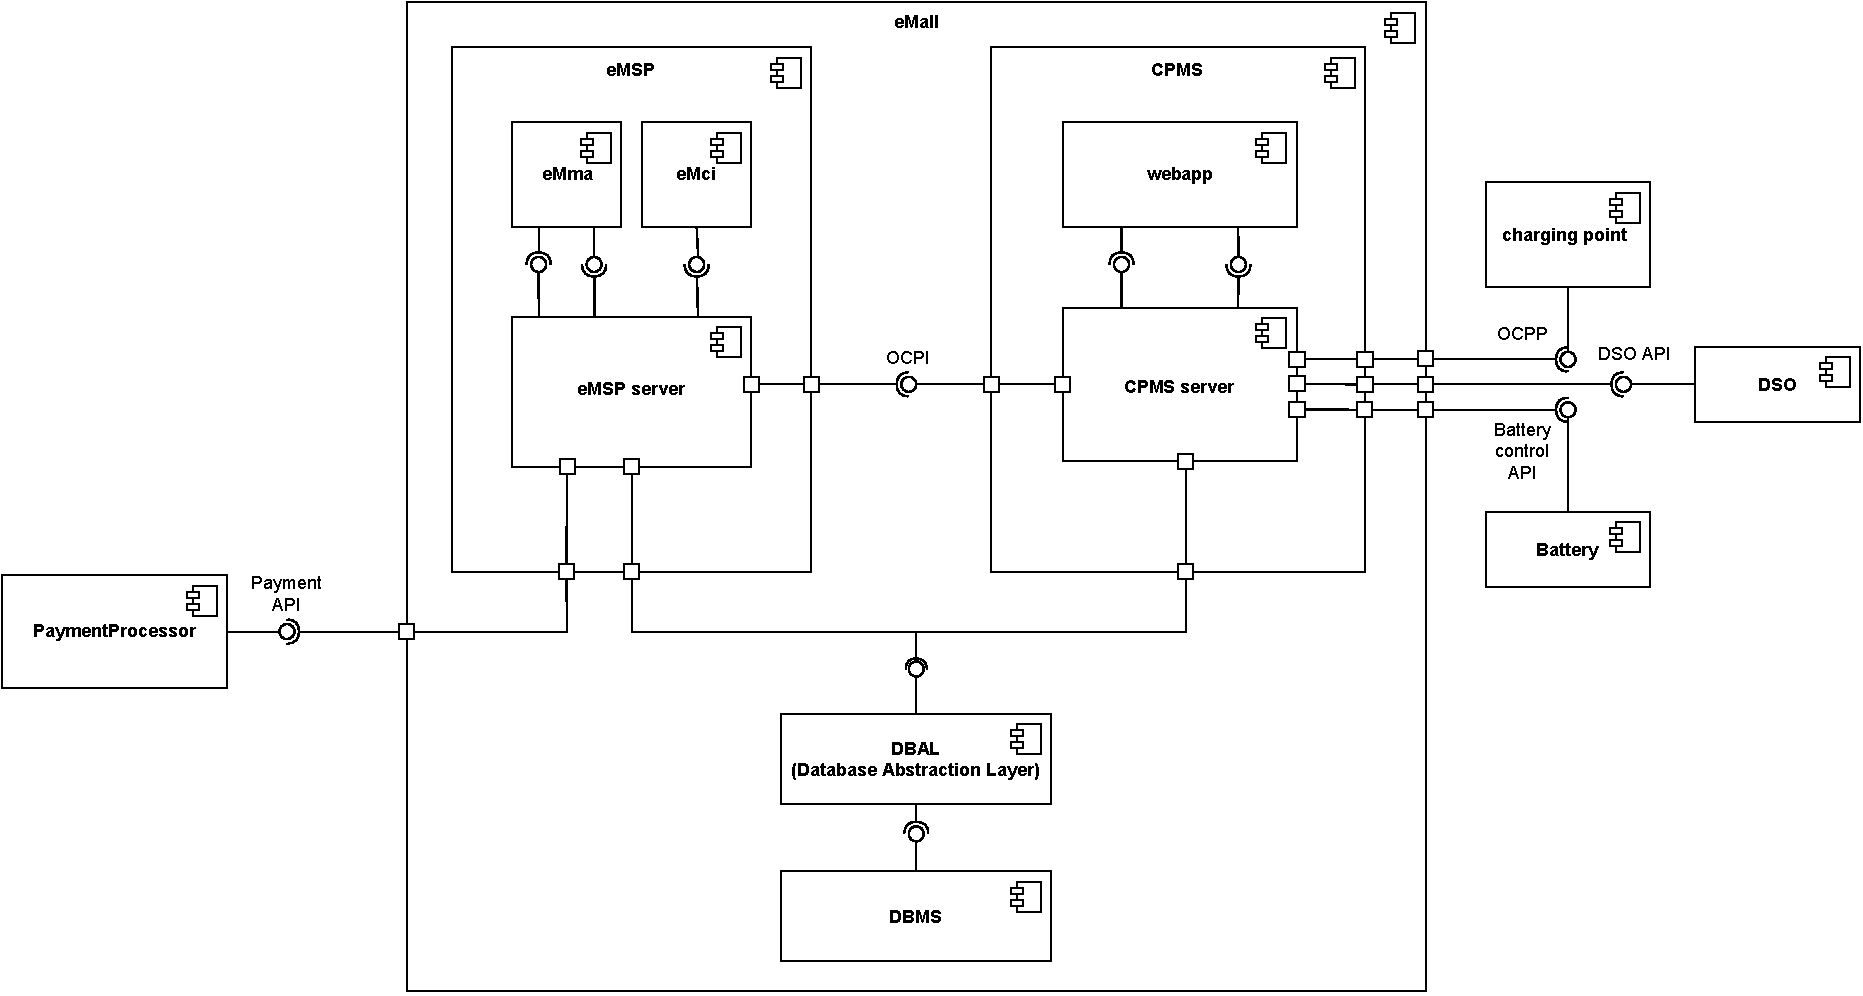
\includegraphics[width=1\textwidth]{Images/cp2/component_overview.pdf}
    \caption{Component view of the system}
\end{figure}

This component diagram provides a higher level view of how the system is composed. It distinguishes the parts that the development team must build (the eMall component), and lists the external system with their respective interfaces with which the eMall must interact to provide its functionalities. Furthermore, it's apparent that the system is composed by two main sub-systems, the eMSP and CPMS, that must interact with each other through the OCPI interface, and each one of these sub-systems is structured with a client-server architecture. The OCPI interface is an open and free interface that standardizes the interface of a CPMS, in other words it standardizes the services a CPMS offers and how to make requests for these services to the CPMS. As a consequence of using the OCPI protocol we allow our eMSP to be able to interact with different CPMS\textit{s}, and our CPMS to interact with different eMSP\textit{s}, as per requirement. Finally, there are the DBMS and DBAL components, that compose the third and bottom tier of our architecture. The presence of the DBAL component tells us that a level of indirection from the DBMS has been added, allowing the system to be independent from any particular DBMS. Regarding the external components with which the eMall shall interact we denote with \textit{Central Electrical System} the software system responsible for managing the technical aspect of the charging station, like unlocking the charging point, controlling the flow of electricity at a charging point and connecting (likewise disconnecting) electrical components to the electrical. With Battery we denote the software responsible for managing the battery, like monitoring the charging status or the level. Next, there is the DSO, with denotes the software system of DSO that will be used by the CPSM, to gather information about energy price and conclude electricity purchase contracts. Finally, there is the PaymentProcessor to which the eMSP will forward the payment request from the user to pay for the charging sessions.
\par
In the next paragraphs we shall discuss in more detail the composite structure of the main sub-systems of the eMall: the eMSP and CPMS.
\pagebreak

\textbf{eMSP}\\
\begin{figure}[H]
    \centering
    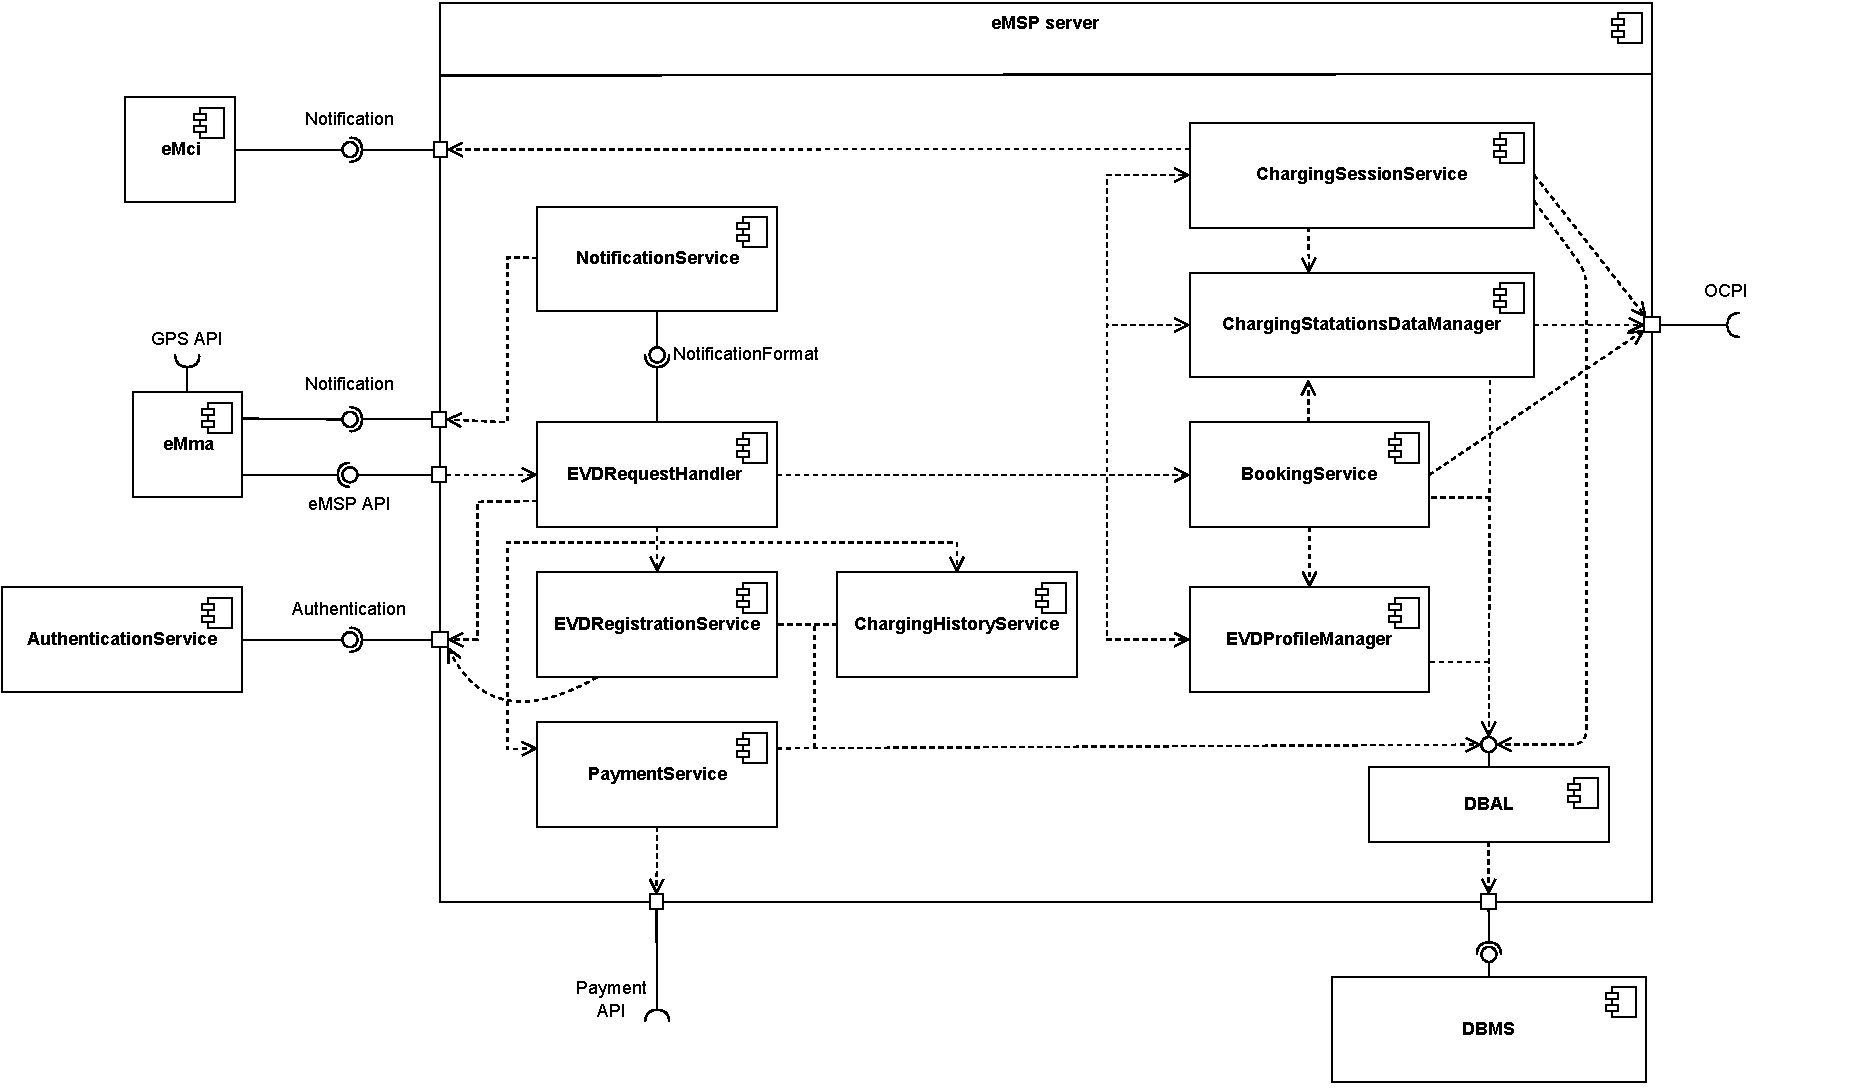
\includegraphics[width=1\textwidth]{Images/cp2/eMSP_server.pdf}
    \caption{eMSP composite structure}
\end{figure}

The eMSP is the system that will interact with the EVD and forward his charging request to the CPMS. As we can see the eMSP isn't only a middleman between the EVD and the CPMS but offers other services like profile management, payment services and charging history services. Below we provide a brief description of each component of the eMSP:
\begin{itemize}
    \item \textbf{eMma}: eMall mobile app. It is the client componet of the eMSP, and its task is to act as a view and partially as a controller for the EVD interactions. Specifically, it will provide a GUI to the user from which he can make his requests to the eMSP. Furthermore, it will encode the user input and interaction with the view to the corresponding functions of the eMSP server interface. Finally it has to interact with the GPS module of the OS in which it will run to provide location information to the eMSP
    
    \item \textbf{eMci}: eMall charging interface. This component's role is to provide the graphical interface the EVD will be using at the charging point when he wants to start a charging session and is located on an embedded device on the charging point. Its job is, then, to identify the charging point in which it resides so the EVD can inform the eMSP of which charging point he wants to use

    \item \textbf{DBMS}: Database Management Service. It is the usual system with the task of managing the insertion, storing, deletion and update of the data generated by the system. This component is exceptionally complex and given the widely availability of this kind of systems on the market, using an already build and thoroughly tested one will be mandatory

    \item \textbf{DBAL}: Database Abstraction Layer. It functions as an additional layer of indirection form the DBMS. In this manner the eMSP will be independent of the DBMS used and if this component changes in the future the eMSP won't need to be modified to integrate the interface of the new DBMS

    \item \textbf{AuthenticationService}: Component that has to mange user's authentication to the system and authorization to use the services

    \item \textbf{PaymentService}: This component, through the usage of external Payment APIs offered by external providers, allows the eMSP to handle the payment requests from the users

    \item \textbf{ChargingHistoryService}: The component which has to process the data saved in the DB to present the user with a functional information regarding his charging history

    \item \textbf{EVDRegistrationService}: Component which has to handle the user registration process. Obviously it shall use the DBAL to store the user information once the process has finished. Additionally it also has to use the component AuthenticationService in order to login the user once the registration process has successfully ended

    \item \textbf{EVDProfileManager}: Component responsible for managing and processing the data concerning the EVD personal information and the EVD's data about his EVs

    \item \textbf{ChargingStationsDataManager}: This is one of the main components of the system. It has to interact with the CPMS to gather data useful for the EVD and more specifically that will be used and processed by the other components. Moreover it acts as an interface for other components that need information about the stations, so they do not need to depend on the data structure used to store the stations

    \item \textbf{ChargingSessionService}: Component responsible for unlocking the charging point, starting the charging session and terminating it. Obviously to offer this services it must interact with the CPMS through the OCPI interface. Additionally it uses the DBAL interface in order to save the data about the charging session, which will be used by the ChargingHistoryService component, and can perform checks when the user is trying to unlock the wrong charging point by cross-checking the data stored in the DB about the charging points and the code it receives by the eMci component

    \item \textbf{BookingService}: Component that provides the booking functionality. It must use the EVDProfileManger and the ChargingStationsDataManager components to get the specific information about the user and the station respectively in order to make the appropriate request through the OCPI interface. Moreover it stores this information in the DB so it can next be used if necessary to cancel a booking
    
    \item \textbf{NotificationService}: Component that provides the eMSP server with the capability of sending notification to the EVD through the eMma component, consequently this component must use the communication interface offered by eMma

    \item \textbf{EVDRequestHandler}: All the users' requests pass through this component. This centralized approach is need so the system can check if the requests have the right permissions (i.e. request for services allowed only for registered user). This explains the dependency with the AuthenticationService component. Obviously it also need to use all the other components to grant the user the services offered by the system

\end{itemize}
\pagebreak

\textbf{CPMS}\\
\begin{figure}[H]
    \centering
    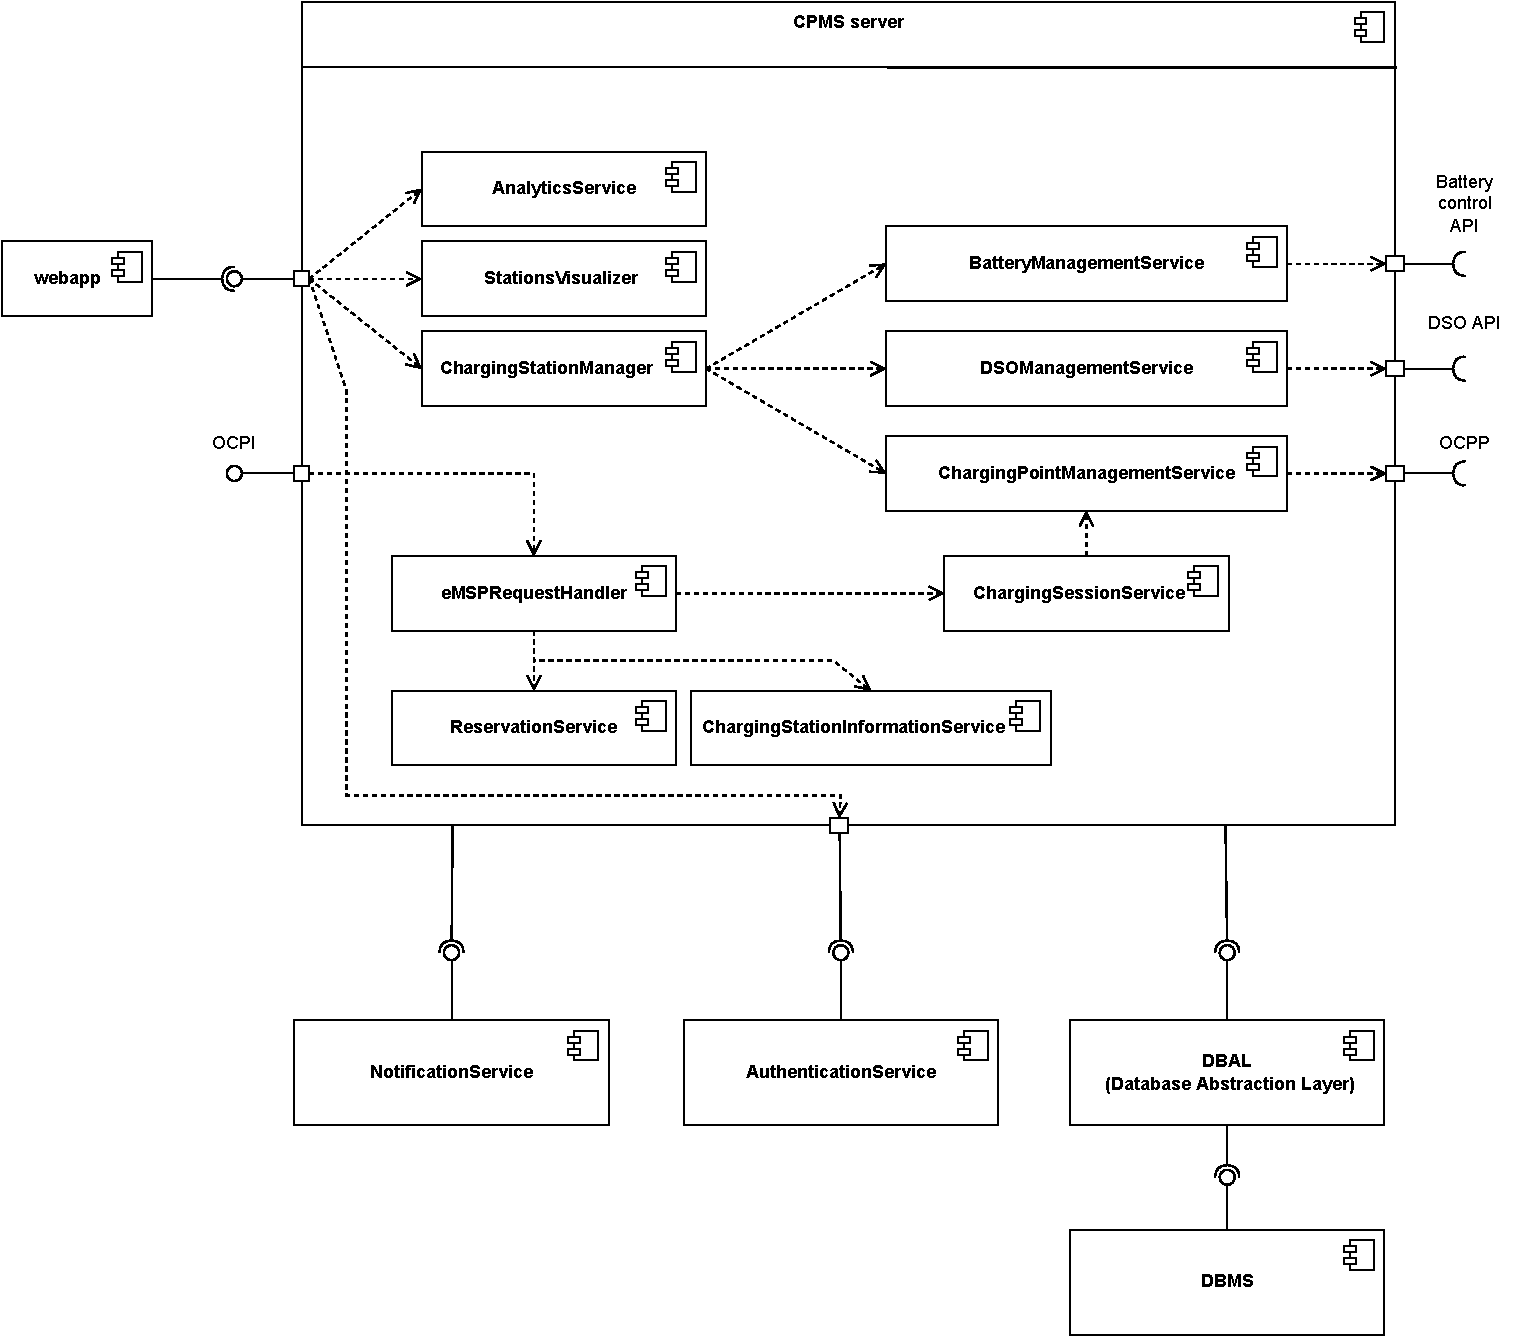
\includegraphics[width=1\textwidth]{Images/cp2/CPMS_server.pdf}
    \caption{CPMS composite structure}
\end{figure}

The CPMS is the subsystem responsible for managing the charging stations, offering charging services to EVDs and securing the electricity supply from the DSOs. To offer all this functionalities this sub-system of the eMall must collaborate with other systems external to our own, which can be viewd in the general overview. Specifically, the CPMS needs to interfaces to the system responsible of managing the battery by the \verb|Battery control API| interface, with the DSO IT system through it's API and with the the system managing the charging points devices through the protocol OCPP, which is an open standard. Like we have done for the eMSP, we will proceed describing each component of the CPMS sub-system (components AuthenticationService, DBAL, DMBS and NotificationService have the same functionality as in the eMSP system and shall not be repeated here):

\begin{itemize}
    \item \textbf{CentralManagementSystem}: Component responsible for interacting with the central electrical system of the charging station. This component will query the central electrical system through the OCPP protocol, asking for the status of the charging points, and invoking request like starting (likewise terminating) the flow of electricity of a particular charging point to start a charging session

    \item \textbf{DSOManagementService}: Component responsible for collecting the data from the various DSO and concluding sales contracts with them if the API allows it

    \item \textbf{BatteryManagementService}: Component responsible for managing the battery of the charging station if one is present. This component must interface with the software system managing the technical aspects of the battery through its control API (here called Battery control API) and must use the methods provided by the CentralManagementService component to allow the central system to switch to the battery for charging or charging the battery when requested

    \item \textbf{StationsVisualizer}: Component that allows the CPO to visualize and select one of the charging stations managed by him

    \item \textbf{AnalyticsService}: Component that provides the CPO with the tools to do some statistical analysis on the data collected by each charging station

    \item \textbf{ChargingStationManager}: Main component responsible for the interaction with the CPO. It implements all the functionalities related to the business aspect of the charging station (setting electricity price, promotions, etc.) and uses the components described before for managing the technical aspects of the charging station. This component also uses the NotificaionService component to notify the CPO about any necessary information

    \item \textbf{CPORequestHandler}: It is the component where all the CPO requests must first pass through in order to perform security checks and allow only authorized users to access the services of the CPMS. To offer this functionality the component makes use of the AuthenticationService component to login the user and to check if the requests coming from the webapp have the necessary authorization. If a request passes the controls it's forwarded to the respective component

    \item \textbf{ChargingStationInformationService}: Component in charge of processing the data of the charging station, stored in the DB, in a suitable format for the eMSP and compatible with the OCPI interface

    \item \textbf{ReservationService}: Component responsible of managing the reservation of the charging points 

\end{itemize}

\section{Deployment view}
\begin{figure}[H]
    \centering
    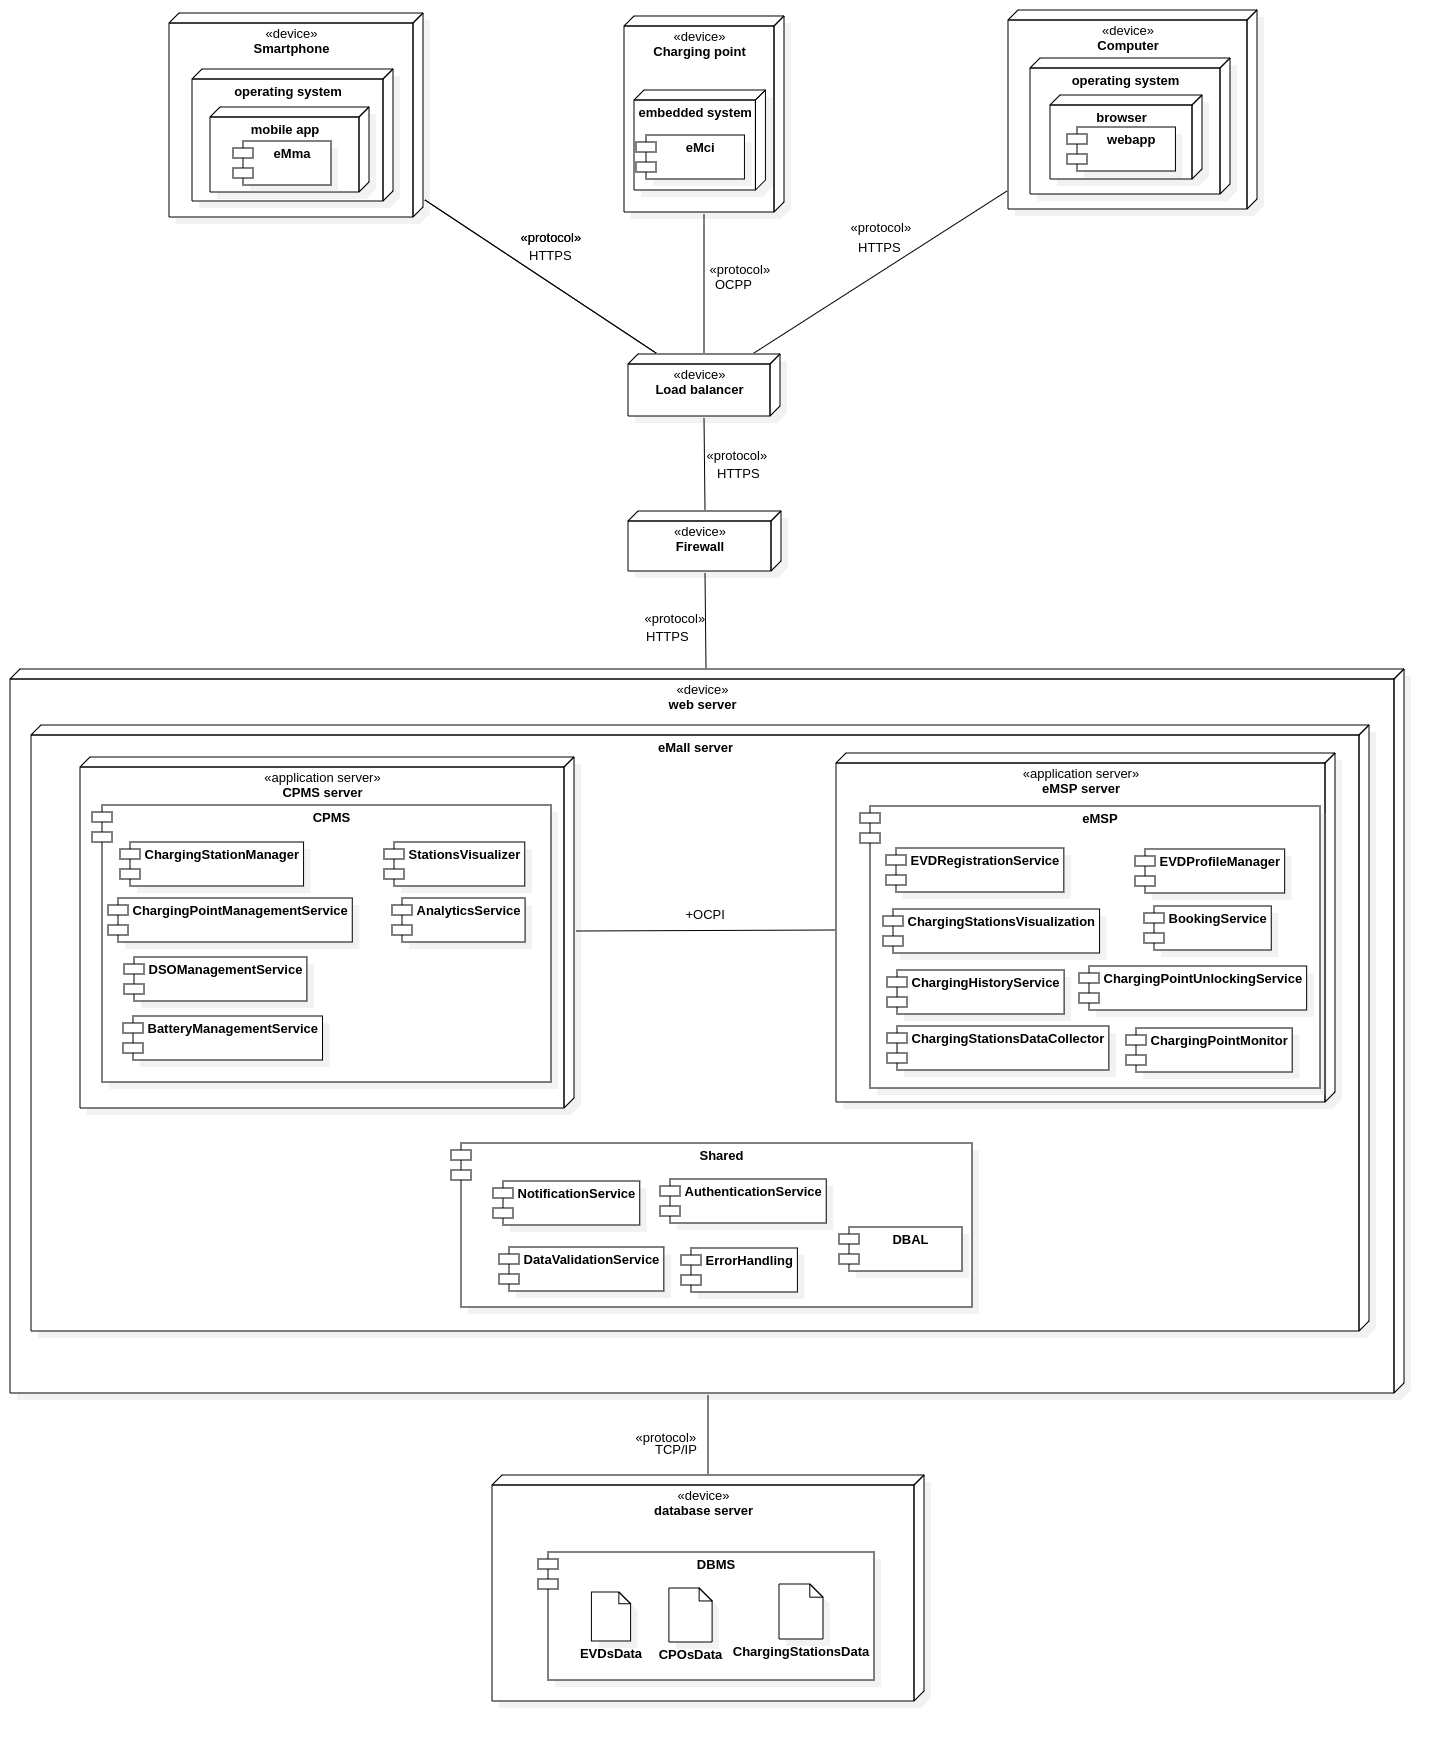
\includegraphics[width=1\textwidth, height=0.9\textheight]{Images/cp2/DeploymentDiagram.png}
    \caption{Deployment view of the system}
\end{figure}
At the client level we can see three different devices interacting with the system:
\begin{itemize}
    \item \textbf{Smartphone} - The smartphone runs the mobile application of the eMall (the eMma) and has internet access in order to send the HTTPS requests to the system. This is the kind of device used by the EVDs that use the eMall
    \item \textbf{Computer} - The computer runs the web application of the eMall, and also has internet access to manage the service through HTTPS requests to the system. This is the kind of device used by the CPOs of the companies that use the eMall to manage their charging stations
    \item \textbf{Charging Point} - The charging point is the specific device used by the EVDs to charge the EVs and it has an embedded system, which through the OCPP protocol communicates with the CPMS part of the eMall system, in order to correctly provide the charging service
\end{itemize}

Between the client level and the application level, we have some architectural elements that allow to achieve some non-functional requirements, such as better performance, scalability, availability and security:
\begin{itemize}
    \item \textbf{Load balancer} - The load balancer is a network device that distributes incoming requests across a group of servers to help improve the performance and availability of the application. A load balancer can help to improve the performance of the application by distributing incoming requests across multiple servers, rather than routing all requests to a single server. This can help to prevent any single server from becoming overloaded, which can improve the overall responsiveness and performance of the application. A load balancer can make it easier to scale the application horizontally by allowing to add or remove servers as needed and this can be useful if we need to add more capacity to handle a growing number of users. A load balancer can, also, help to improve the availability of the application by routing traffic to a healthy server in the event that one of the servers becomes unavailable. We can see that the load balancer is useful to improve different non-functional requirements of the eMall, that can be implemented using different servers to have better overall characteristics 
    \item \textbf{Firewall} - The firewall allows to protect the network from external threats and unauthorized access, blocking incoming traffic that does not meet the security rules. The firewall is necessary in order to comply with certain regulations and industry standards, because we are handling sensitive data (financial information, personal data), so is necessary to protect the data
\end{itemize}

The eMall web application and mobile application provide both static and dynamically generated content, so the system runs web servers for the static content and application servers to generate content dynamically. The load balancer sends to the web server the HTTPS requests that need only static content, and on the other side sends to the correct application server the requests to generate the dynamic content and accomplish more complex functionalities due to the interaction of the eMall components. 
At the application level the deployment diagram shows in a simplistic way the following elements:
\begin{itemize}
    \item \textbf{Web server} - For the web server we have a computer that stores software and website raw data, such as HTML files, images, text documents, and JavaScript files. The hardware of the web server is connected to the web and supports the data exchange with different devices connected to the Internet
    \item \textbf{Application server} - In the deployment diagram on the same hardware we also have the application servers, one for the CPMS and one for the eMSP, with also the shared services. The application servers contain different micro-services, that interact among them and with external APIs, as shown in the previous component diagram. The micro-services could also be implemented on more servers, splitting the eMSP and CPMS application servers in more servers, or creating a redundancy of the available services on different machines to improve performance and availability, exploiting even better the load balancer
    \item \textbf{Shared components} - The shared components shown in the diagram are components that belong to the two application servers, but also to the web server. The web server of the eMall handles part of these functionalities, sending the rest to the application servers  
\end{itemize}

Finally at the lowest level we have the persistent part of the system, which interacts with the eMall through TCP/IP over TLS and is hidden to the higher levels due to the use of the DBAL. The Database level is composed by:
\begin{itemize}
    \item \textbf{Database server} - It hosts the database of the system and manages the different data through a DBMS 
    \item \textbf{Database artifacts} - The different database artifacts shown in the diagram represent physical implementations of the DB, an implementation for the data regarding the EVDs, one for the companies and CPOs data and finally an implementation for the data regarding the charging stations and any other related data
\end{itemize}
For a more secure system we consider not only a DB, but also some replicas, distributed on different machines to guarantee more availability, fault tolerance and disaster recovery. 

\section{Runtime view}
In this section a dynamic view of the system is provided, displaying the interactions between the components identified in section \ref{sec:component_view} by mean of sequence diagrams in UML notation.\\
For the sake of conciseness, repetition of interactions that exhibit the same, or similar, behaviour has been avoided, hence, only the most important interactions emerging from the use case presented in the RASD document are shown here. Furthermore, we mainly present the main interaction of the use cases, disregarding the exceptions, which are shown only in some situations to underline important differences in the flow of events.

\pagebreak
\subsection{EVD runtime view}
\textbf{EVDregistration}\\
\begin{figure}[H]
    \centering
    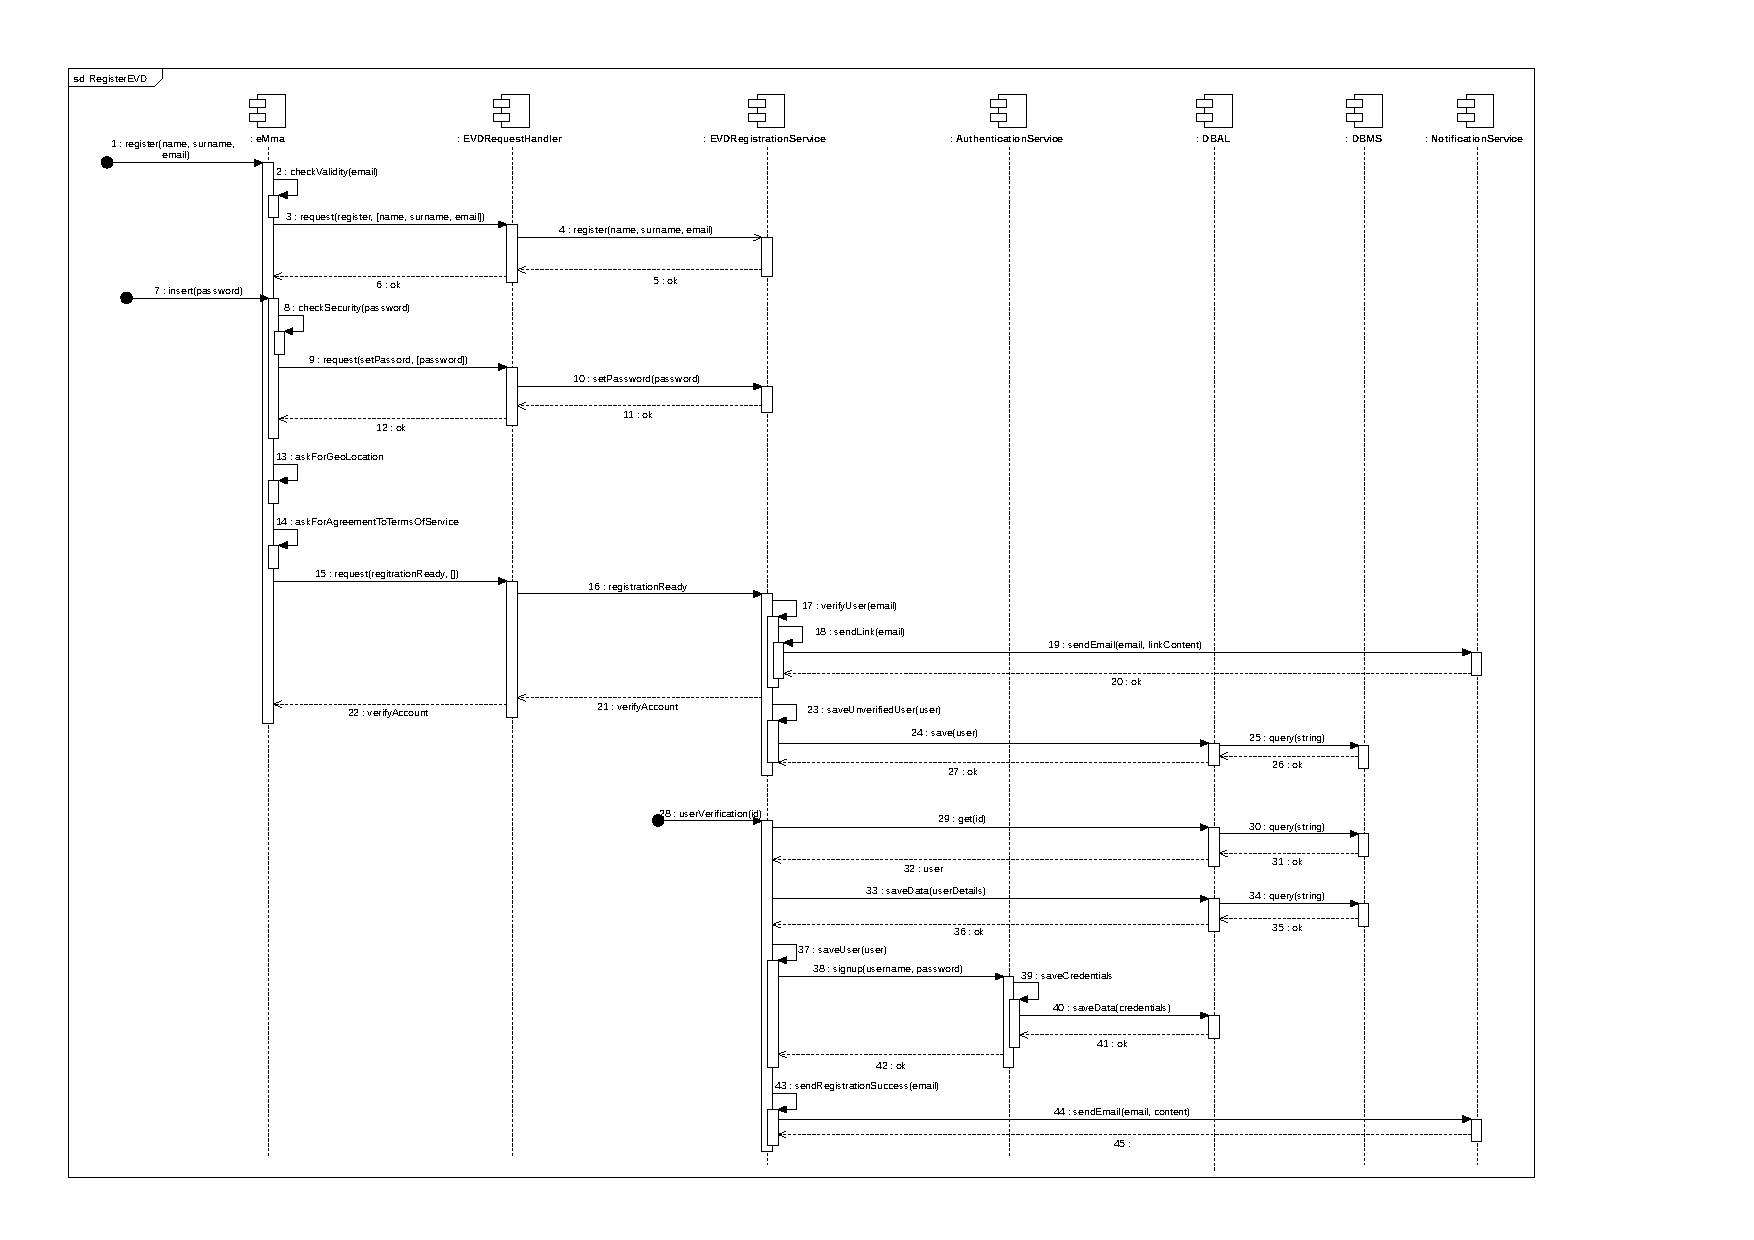
\includegraphics[trim={1cm 1cm 3cm 1cm},clip, width=1\textwidth]{Images/cp2/runtime/EVDRegistration.pdf}
    \caption{EVD registration sequence diagram}
\end{figure}
This diagram shows the interactions taking place between the eMma component, responsible for the interaction with the user, and the EVDRegistrationService, tasked with handling the registration process. As shown in the component diagram (section \ref{sec:component_view}) all the interactions between eMma and the component of the eMSP server must pass through the EVDRequestHandler (ERH from now on) so it can check whether the operations needs special authorization or not. In this specific case the operations do not need any special authorization so the ERH will only dispatch the requests to the right component. The first "found message" represents the user interaction on eMma to start a registration process. eMma, tries first to do a simple check on the validity of the email, by checking if it has the right format. If the controls are successful, eMma starts the interaction with the eMSP server by sending the request with the data to the eMSP server. This request starts the registration process in the EVDRegistrationService (ERS from now on). In this first step the ERS will acknowledge the request and temporary store the data. The next step is for eMma to check for the password when the user inserts it, and then sends the data to the ERS. Next, eMma requests the user to share his geolocation and to agree to the terms of service. If the user agrees eMma sends a message to the ERS to notify him that the data necessary to the registration were gathered. Now the ERS starts a process of verifying the user by sending him an email with a link to verify his data. After he email is sent, the ERS sends the verifyAccount message to eMma and then saves the EVD data into the DB so they can be retrieved later when the user verifies his identity. When the user does so, the ERS proceeds to save the user by asking the AuthenticationService to validate the user. Finally the ERS sends an email to the user notifying him the registration was successfully completed.

\paragraph{Login}\mbox{}\
\begin{figure}[H]
    \centering
    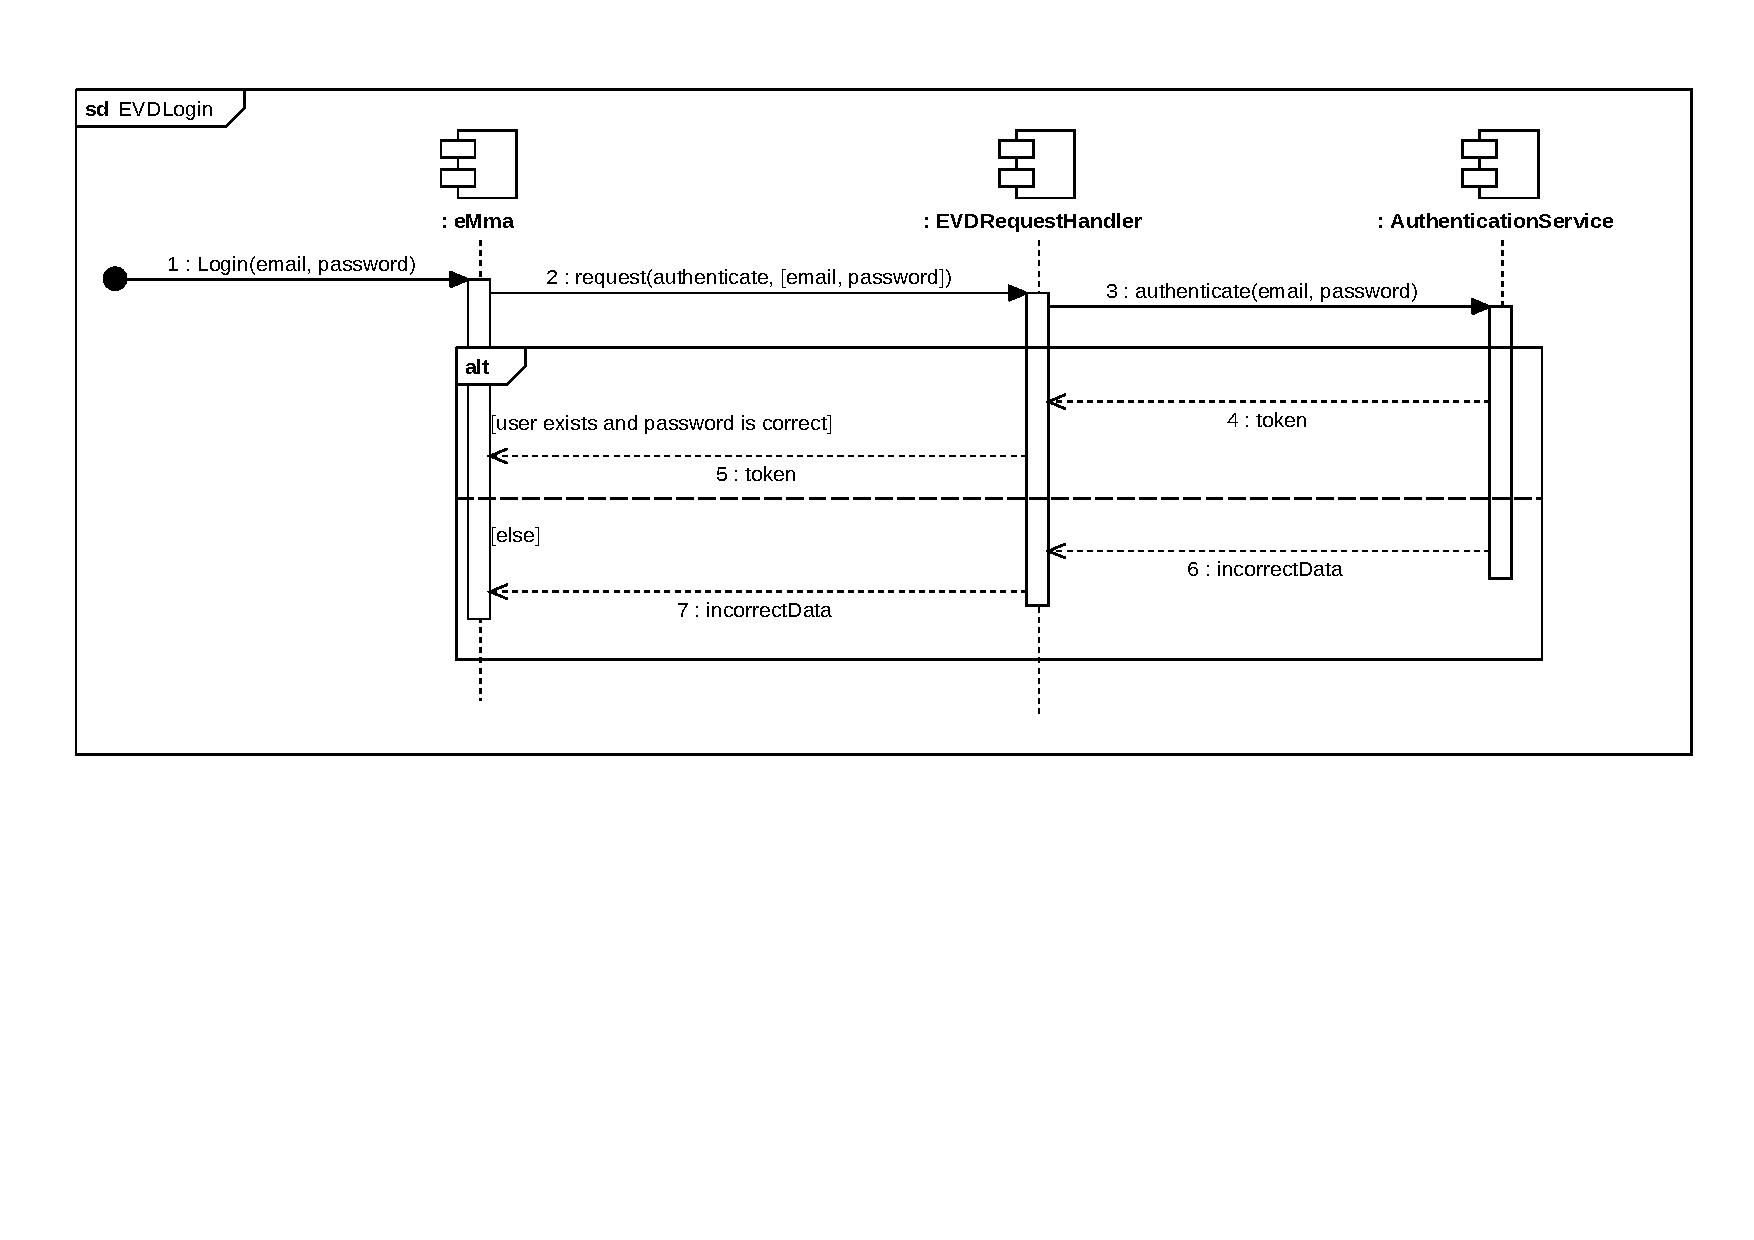
\includegraphics[trim={0 8cm 0 0},clip, width=1\textwidth]{Images/cp2/runtime/Login.pdf}
    \caption{EVD Login sequence diagram}
\end{figure}
This set of interactions is as simple as shown in the diagram. The user starts the interaction by requesting to login in the system and providing the email and password. eMma forwards this request to the eMsp server through the ERH, which passes it to the AuthenticationService. If the email exists and the password is correct then the AuthenticationService returns a token that will be used to access the system services, if not it returns an error message.

\pagebreak
\paragraph{Authorized request}\mbox{}
\begin{figure}[H]
    \centering
    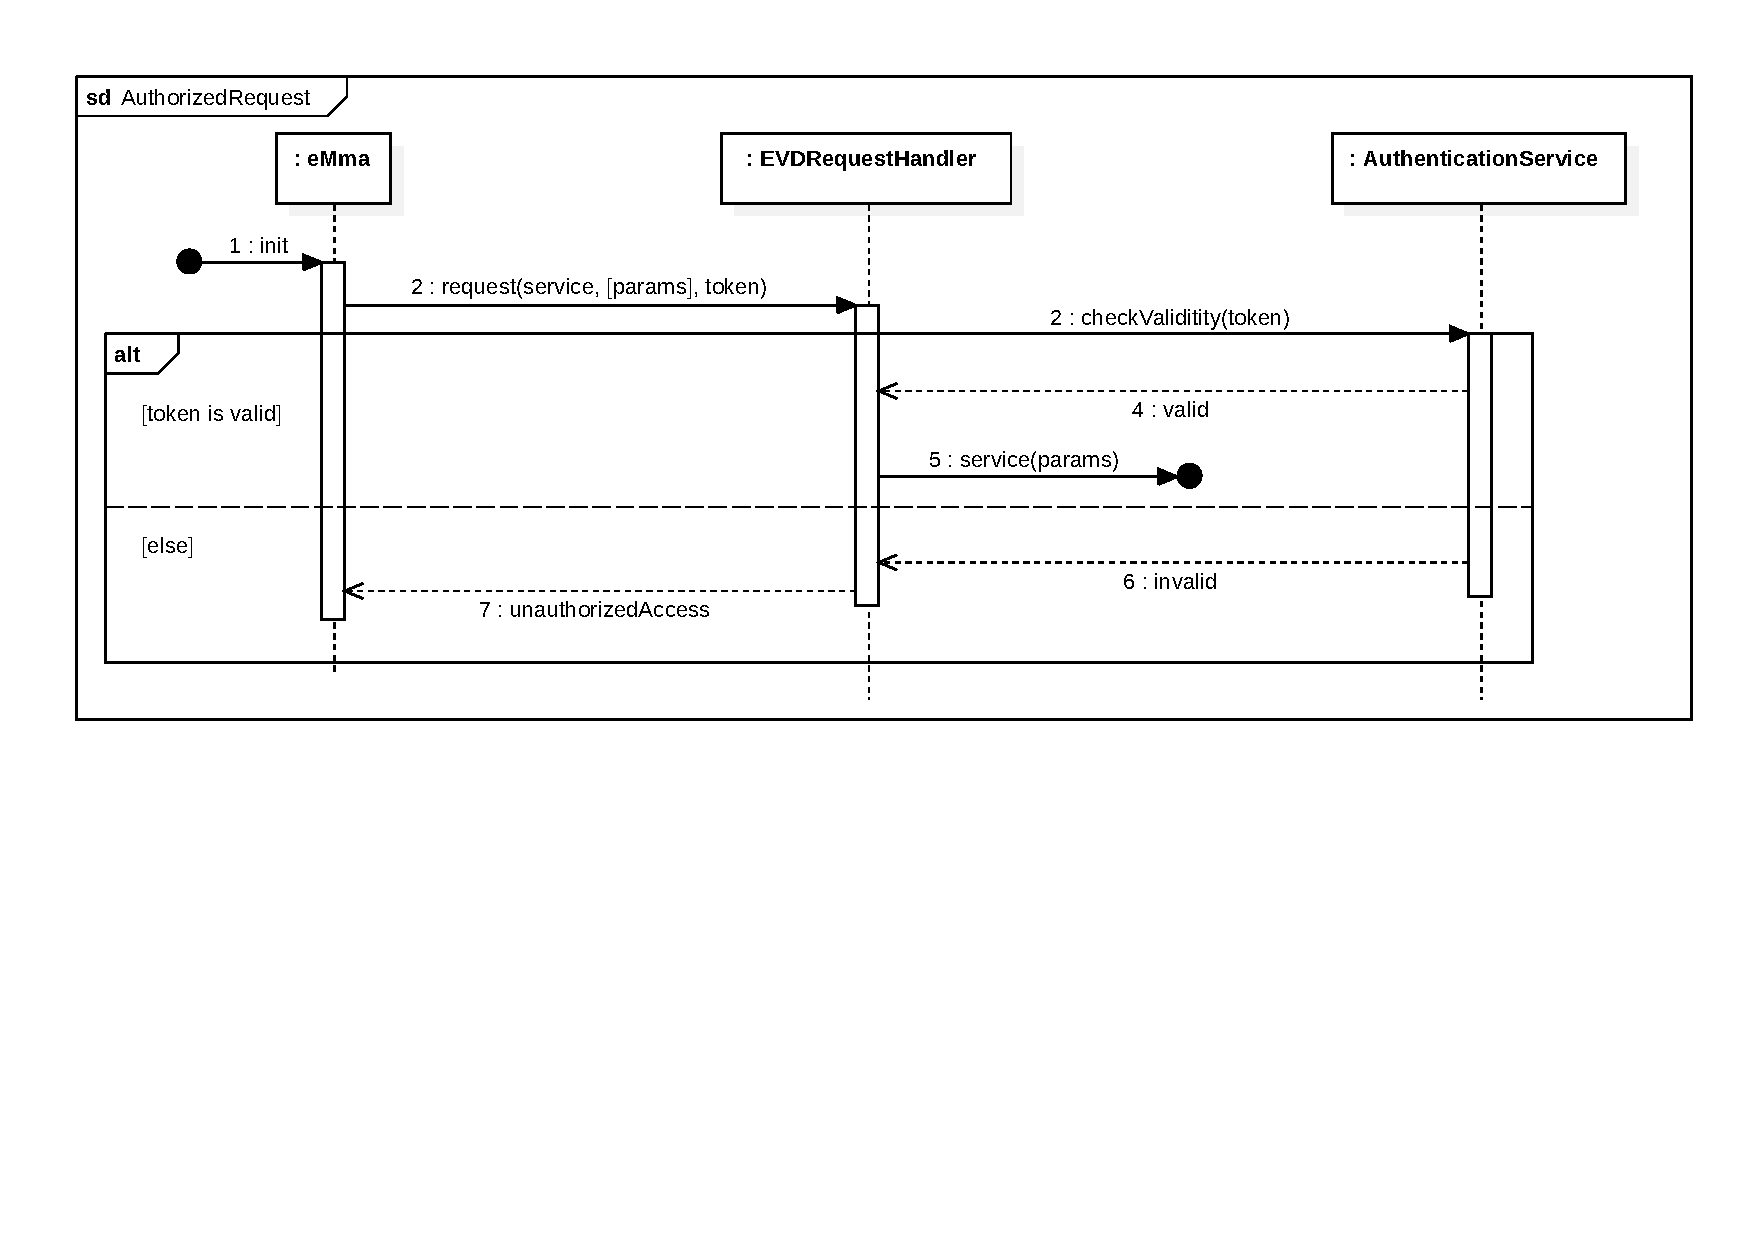
\includegraphics[trim={0 8.5cm 0 0},clip, width=1\textwidth]{Images/cp2/runtime/AuthorizedRequest.pdf}
    \caption{Authorized request sequence diagram}
    \label{fig:auth_request}
\end{figure}
This sequence of interactions doesn't map to any particular use case, but it's an important flow of events that shows how an authorized request is controlled to have the right access permissions. This sequence of interactions will always occur for any authorized request arriving to the system, for both eMSP and CPMS, and for the sake of conciseness it will be considered implicit in the following diagrams. The diagram is left generic precisely because how general this sequence of actions is. As always the interactions start with an outside message that triggers eMma to invoke a service of the eMSP. Along with the arguments needed to request the service, for authorized operations, eMma needs also to yield the token obtained during the login phase. Secondly, the ERH asks the AuthenticationService to check if the token is valid: if it is, then it proceeds to call the methods of the required service with the arguments it received from eMma. If the token is invalid, ERH sends an \textit{unauthorizedAccess} message to eMma.
\pagebreak

\paragraph{Booking}\mbox{}\\
For this interaction we have decided to split the diagrams in two, showing first the interactions that occur in the eMSP subsystem, and afterwards showing the sequence of actions that happen in the CPMS.

\begin{figure}[H]
    \centering
    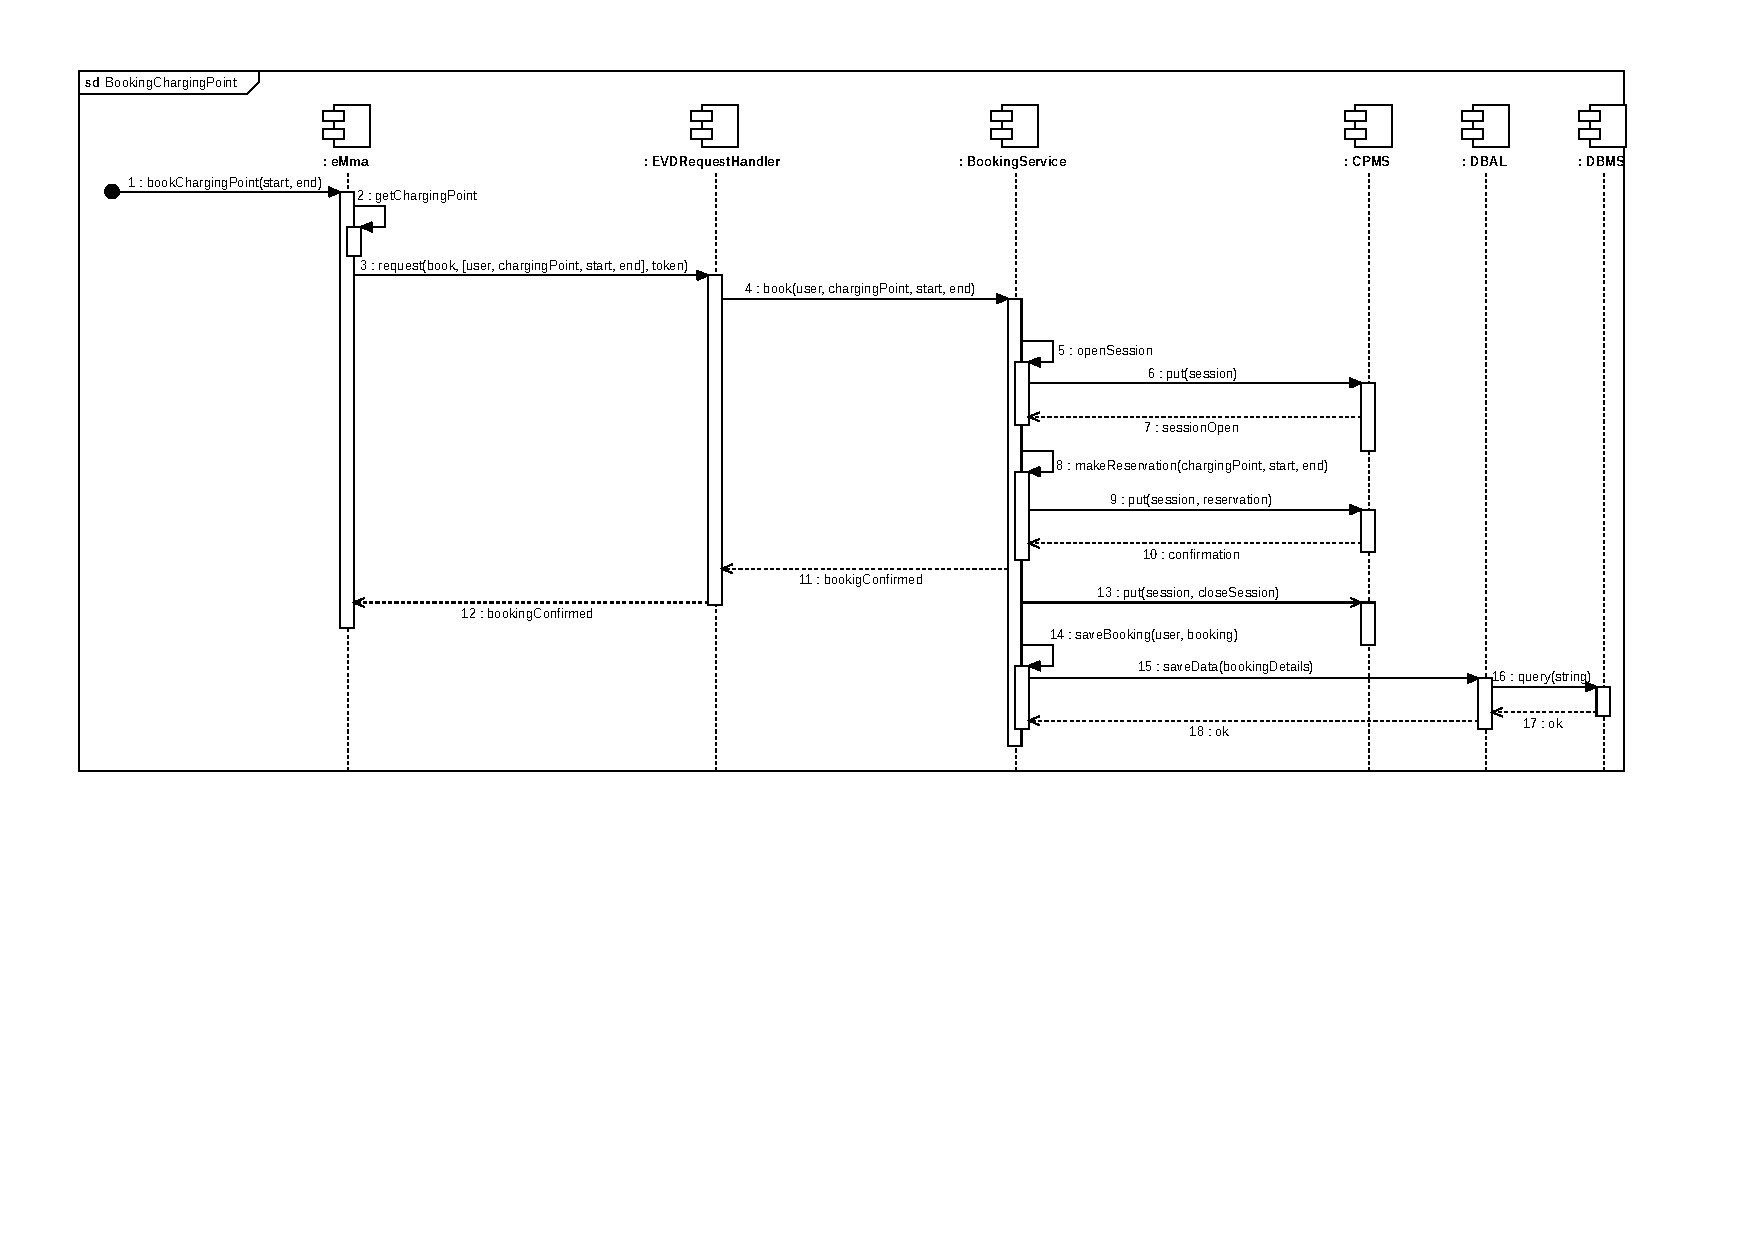
\includegraphics[trim={0 4.5cm 0 0},clip, width=1\textwidth]{Images/cp2/runtime/Booking_emsp_view.pdf}
    \caption{Charging point booking sequence diagram}
\end{figure}
The interaction starts when the user inserts the start time and end time of the booking (notice that this are timestamps, so the date is already encoded). Next, eMma retrieves the data of the charging point the user has selected in the view and sends the request to the eMSP. The request, after validating the token, is forwarded to the BookingService. The latter component must interact with the CPMS to make the reservation. The interactions between the BookingService and the CPMS follow the standard stated in the OCPI protocol. When the reservation is confirmed by the CPMS, the BookingService sees to send the confirmation message back to eMma.\\
\\
From the perspective of the CPMS we show the sequence of actions, considering the session is already started, hence the interactions start from the PUT method from the eMSP making a request for a reservation. The eMSPRequestHandler validates the request analyzing the token embedded in session object (like we have shown in diagram \ref{fig:auth_request}) and then dispatches the request to the ReservationService component, which unpacks the reservation object to extract the data he needs and makes an availability control on the charging point and the time span requested. \\
If the controls are positive then the ReservationService proceeds to send a confirmation message back to the eMSP and saving the reservation in the DB to update the information about the station.
\begin{figure}
    \centering
    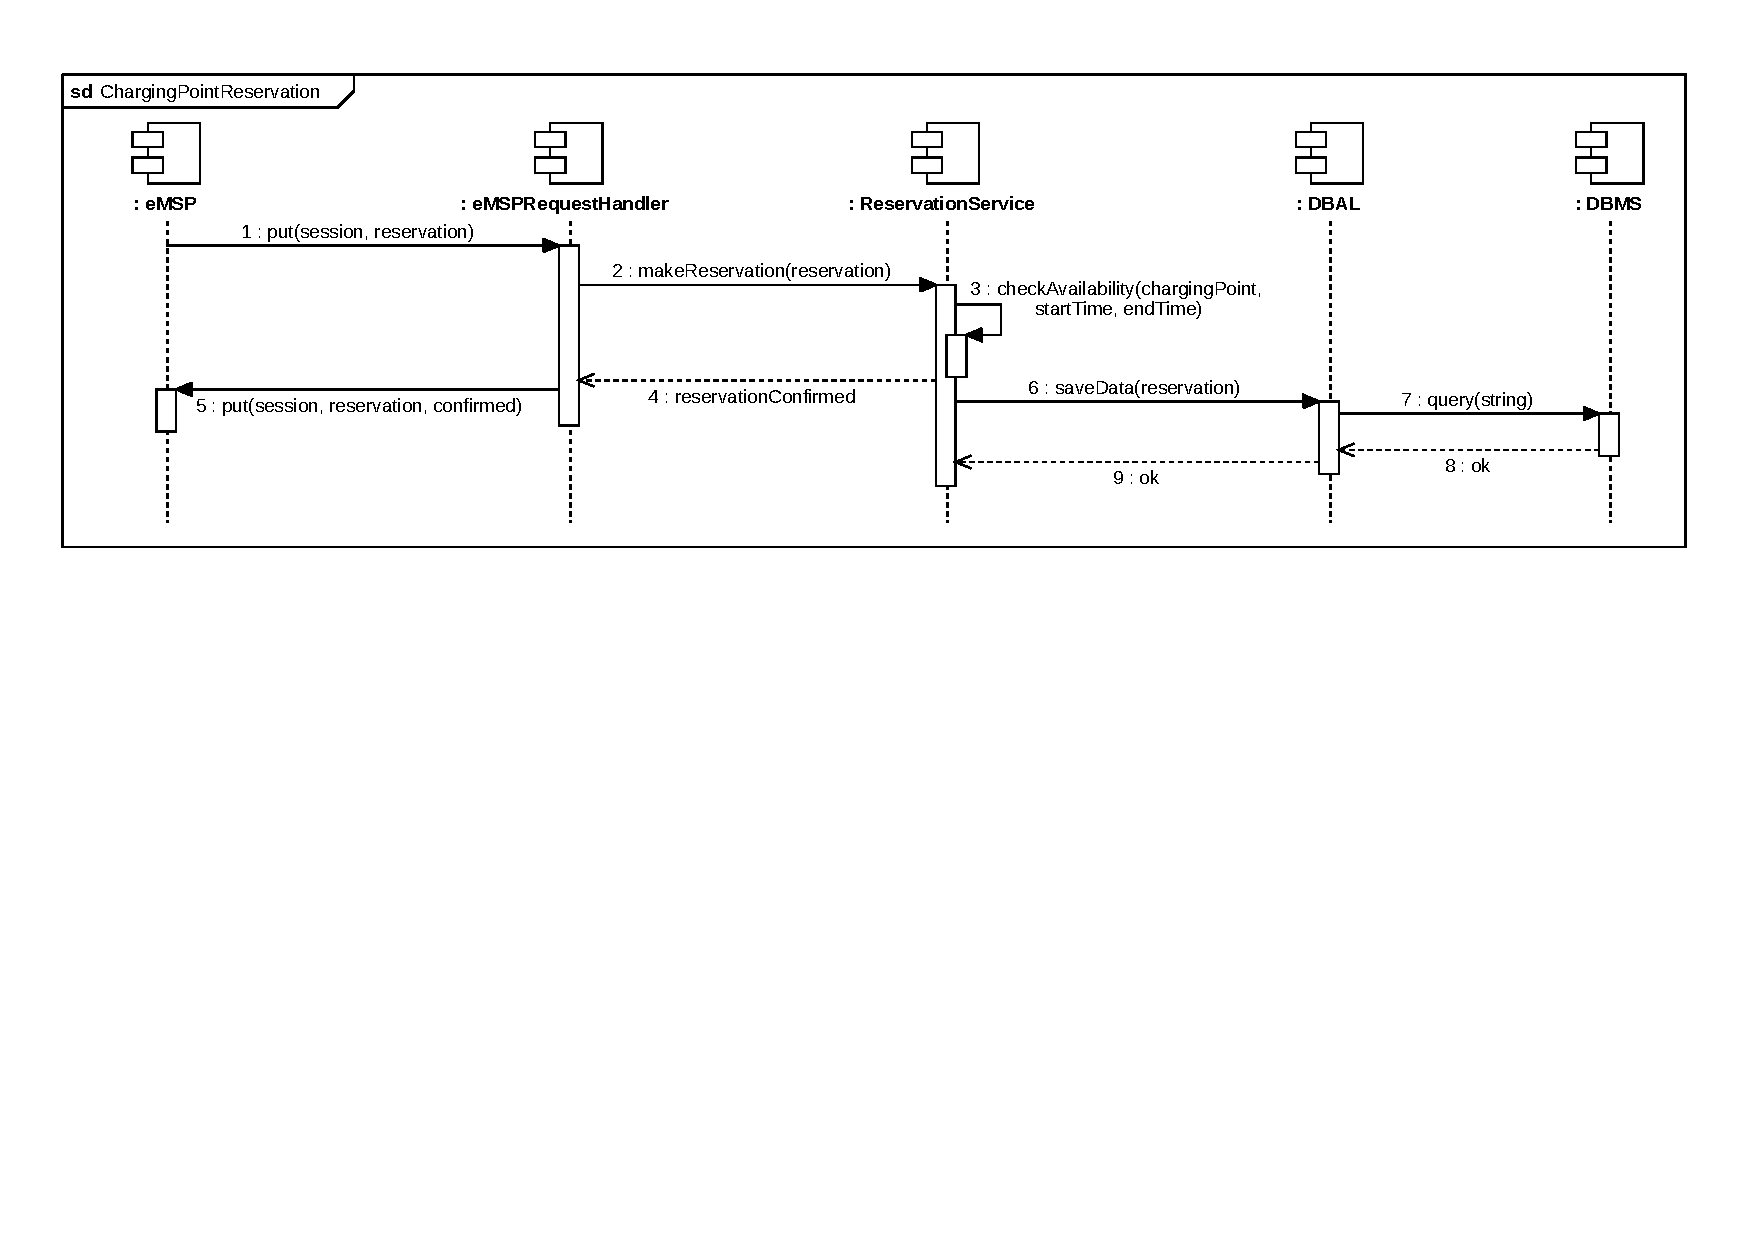
\includegraphics[trim={0 10cm 0 0},clip, width=1\textwidth]{Images/cp2/runtime/Booking_cpms_view.pdf}
    \caption{Charging point reservation sequence diagram}
\end{figure}


\paragraph{VisualizeStations}\mbox{}\\
\begin{figure}[H]
    \centering
    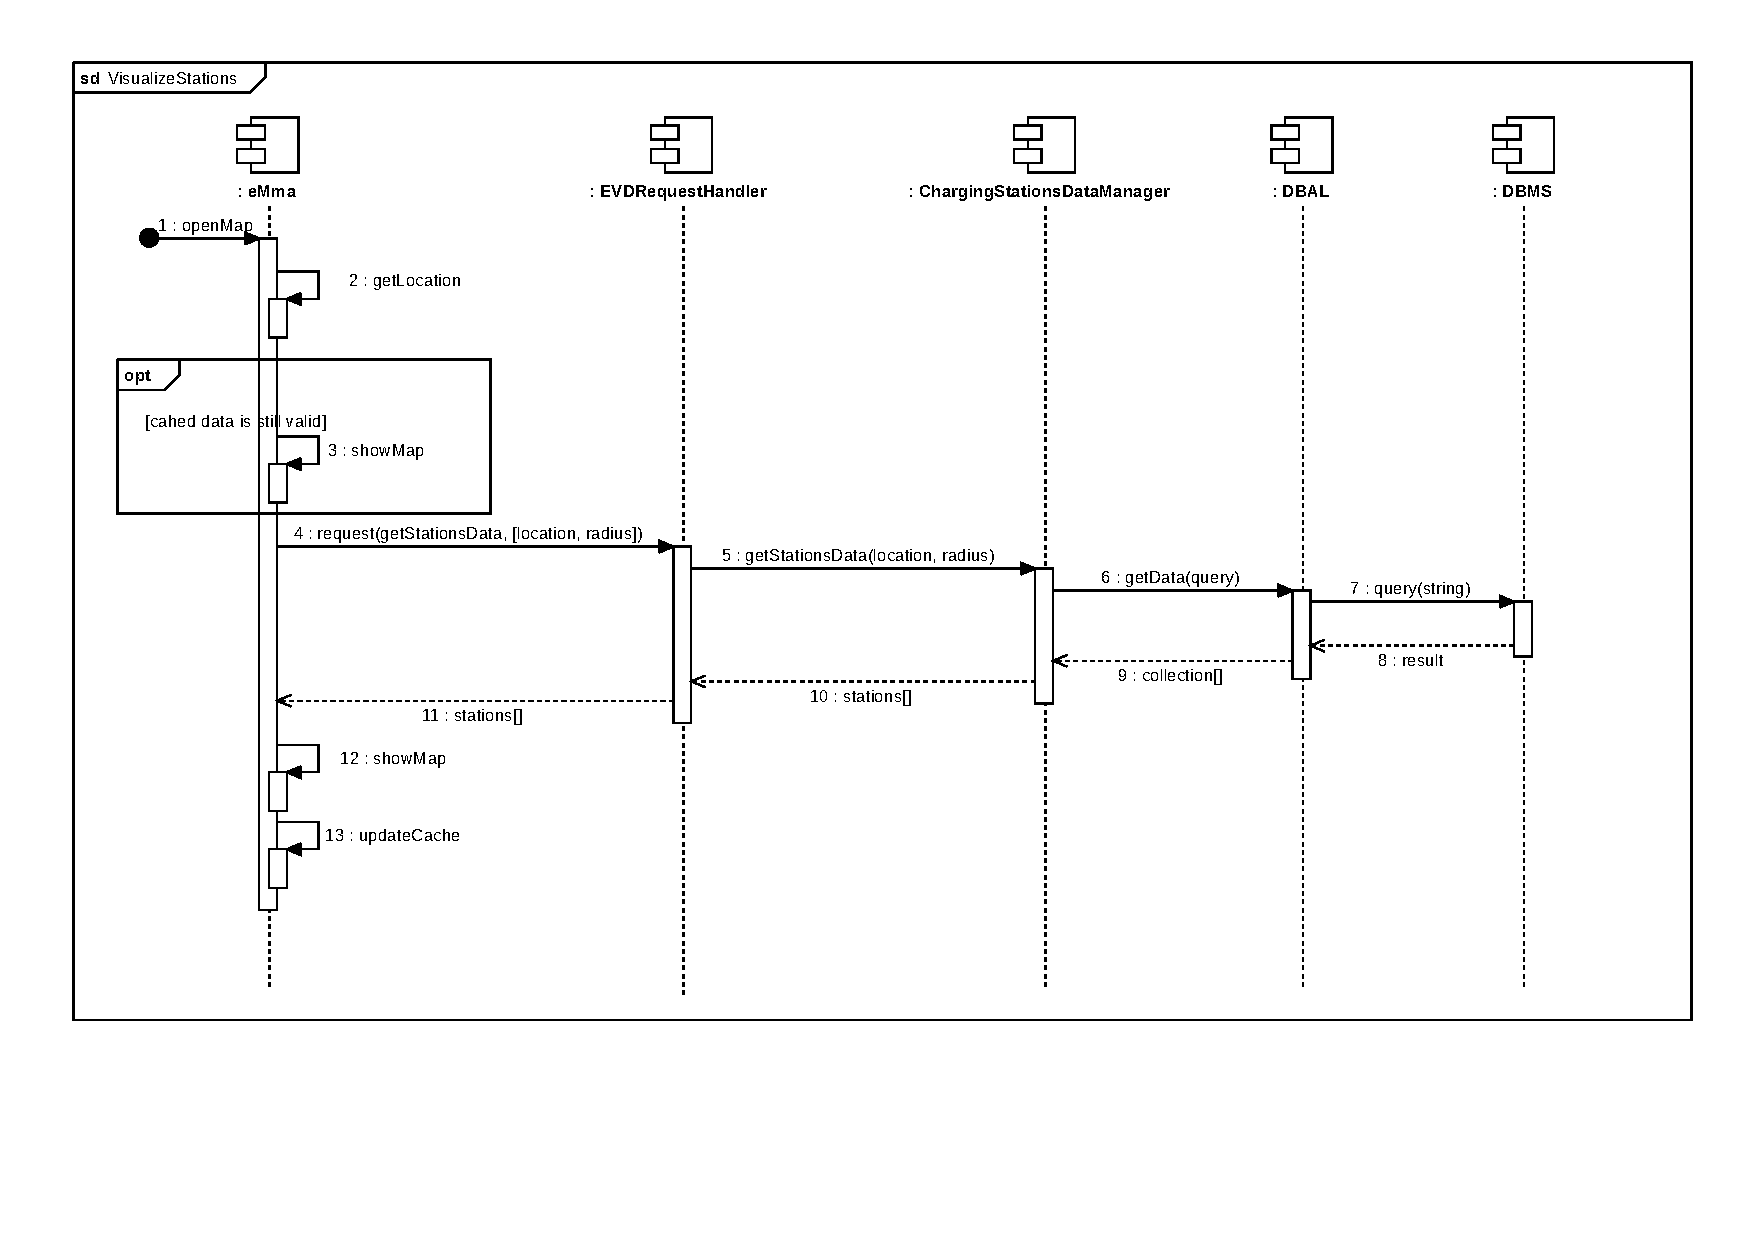
\includegraphics[trim={0 3cm 0 1cm},clip, width=1\textwidth]{Images/cp2/runtime/VisualizeStations.pdf}
    \caption{Visualize stations sequence diagram}
\end{figure}
\pagebreak
The process of visualizing the stations starts when the user opens the app and is greeted with a map. Next, eMma gets the location information from the user smartphone as shown with the self call \textit{getLocation}. Before asking the stations' data to the eMSP server, eMma tries to first check if the data it has cached is still valid and if it is, then it generates the map based on this data. If the cache is invalid, eMma requests to the eMSP server the data about the stations. Please note that the request doesn't need authorization so the token is not passed as an argument. The request is then dispatched to the ChargingStationsDataManager, which through a series of methods call to the DB retrieves the necessary data and returns it back  to eMma.

\paragraph{ChargeNow}\mbox{}\\
The starting of a charging session is an operation that involves the eMSP and the CPMS as well. As we did before we will split the flow events in two, showing fist the interaction from the eMSP point of view, afterward we will display the interactions from the CPMS point of view.
\begin{figure}[H]
    \centering
    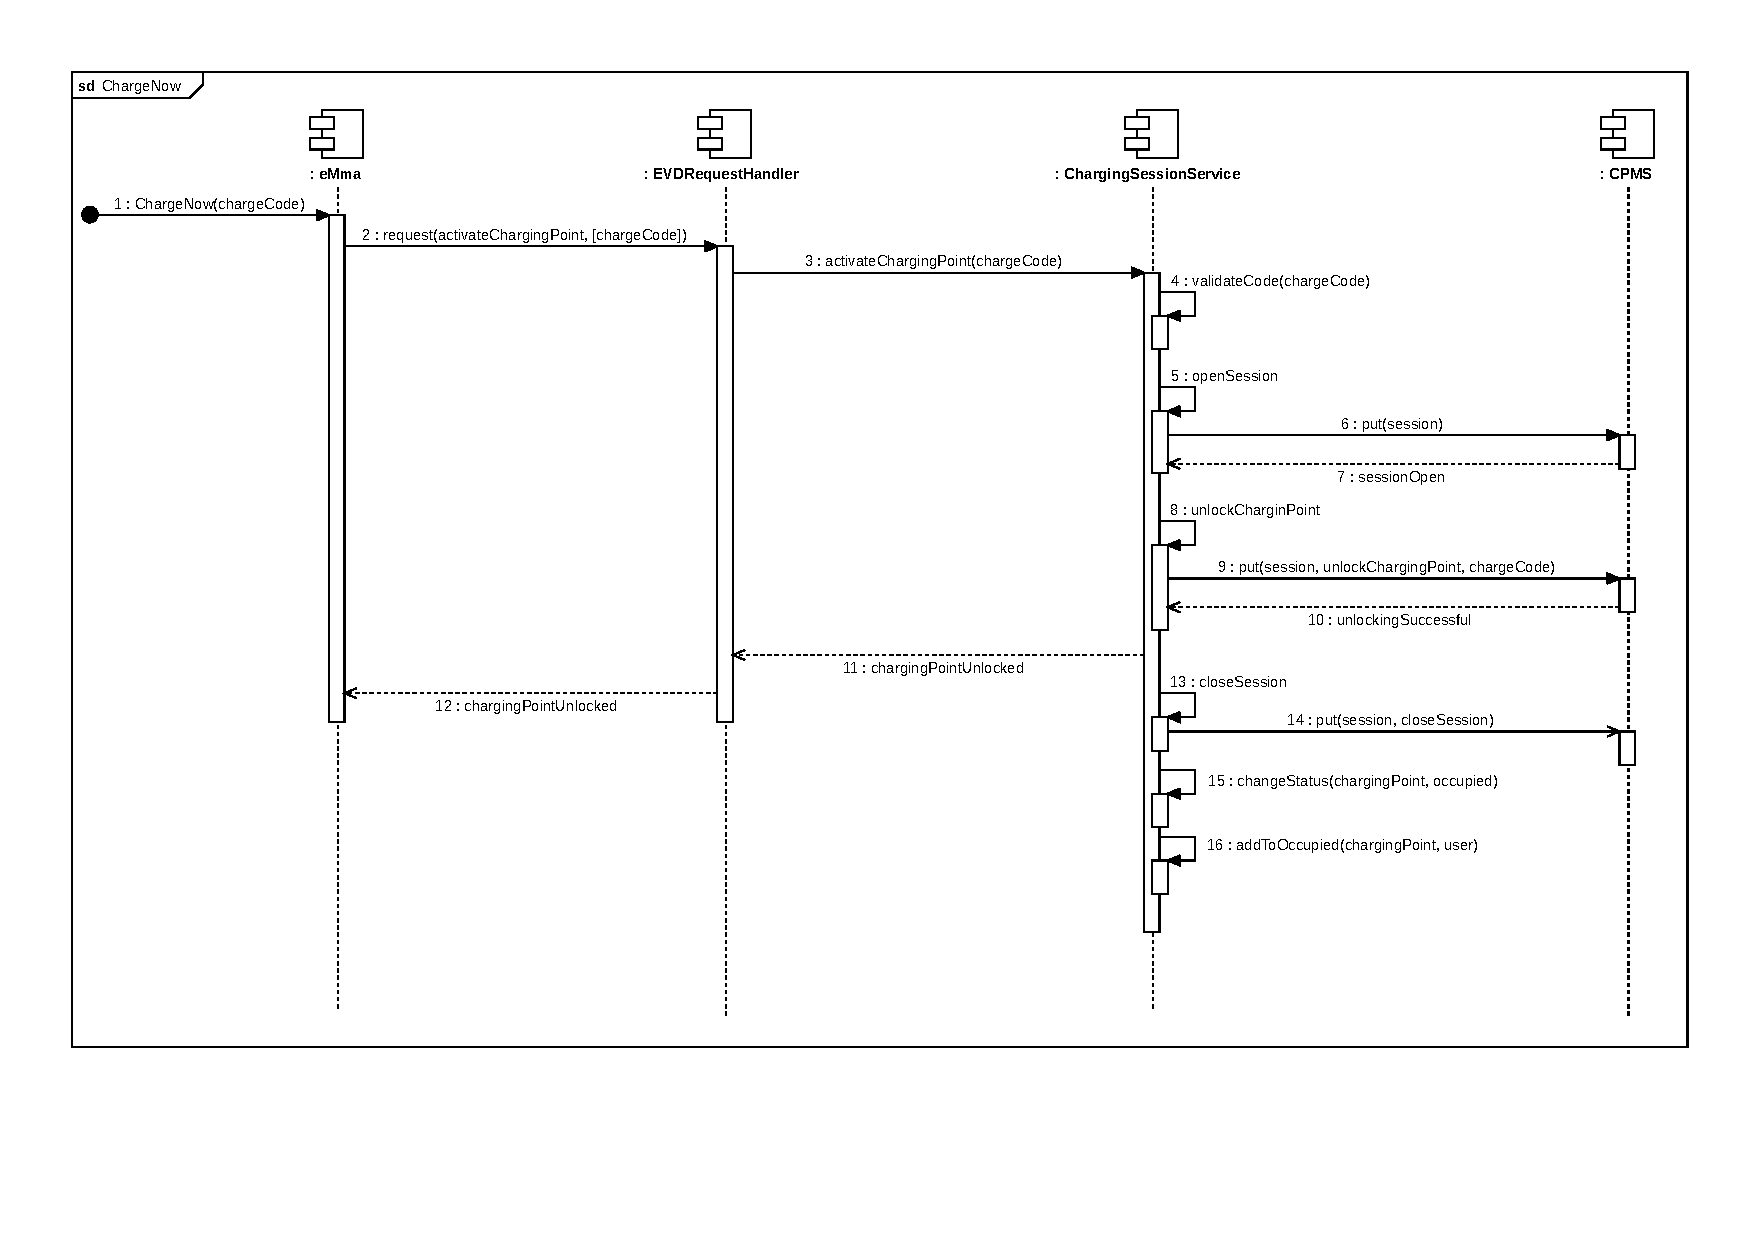
\includegraphics[trim={0 3cm 0 1cm},clip, width=1\textwidth]{Images/cp2/runtime/ChargeNow_emsp_view.pdf}
    \caption{Start Charging session sequence diagram}
\end{figure}
The interaction starts with the insertion of the chargeCode by the EVD, which he gets from the display of the eMci device installed on the charging point. The eMma forwards the request of activating the charging point with the respective code to the eMSP server, which handles it through the EVDRequestHandler. The latter, given the request, invokes the right method on the ChargingSessionService component (CSS from now on). After the method is invoked on it, the CSS performs a preliminary check on the format of the chargeCode and if the chargeCode exist in the system. If the controls pass the CSS opens a session with the CPMS to request the unlocking of the charging point associated with the aforementioned code. This sequence of actions is very similar to the ones already described in the Booking sequence diagram, thanks to the uniform OCPI interface. If the CPMS unlocks the charging point correctly, then the CSS proceeds to send back to eMma the reply message for the correct conclusion of the request. However, the CSS task doesn't end here, obviously he has to close the session with the CPMS but he also needs to change the status of the charging point to occupied and he has to keep record of which user is using which charging point, so it can show the charging status of the EV to the respective EVD.

\begin{figure}[H]
    \centering
    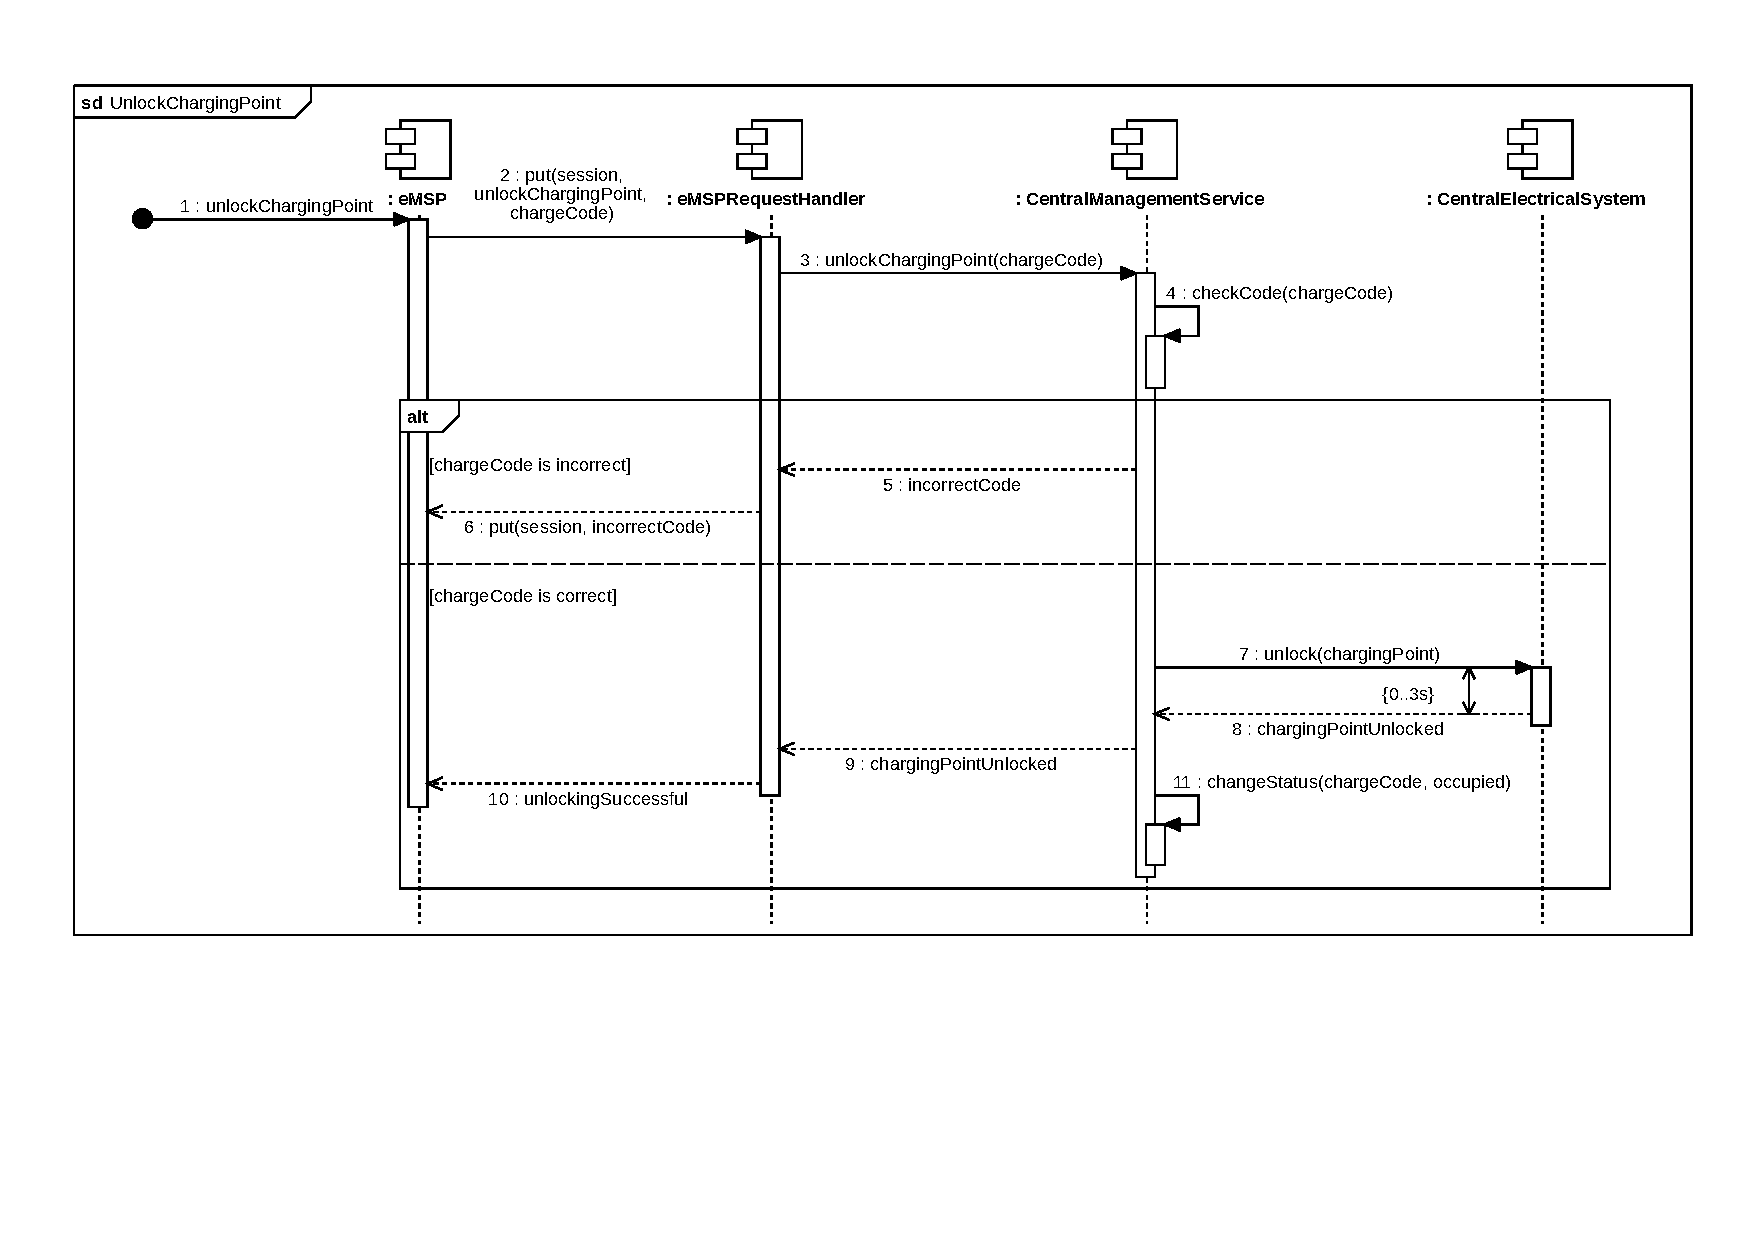
\includegraphics[trim={0 5cm 0 1cm},clip, width=1\textwidth]{Images/cp2/runtime/ChargeNow_cpms_view.pdf}
    \caption{Unlock charging point sequence diagram}
\end{figure}
The diagram starts directly when the CPMS receives the PUT message to unlock a specific charging point delineated by the chargeCode. The request is handled by the eMSPRequestHandler which, after doing all the security checks, dispatched the request to the CentralManagementService (CMS) which is the component responsible for it. The first operation of the CMS is to check if the code refers to a charging point actually present in the station. If this is not true, then an error message is returned. If the test passes, then the CMS starts the operations of unlocking the charging point, which consist of preparing a correct data structure of the charging point, starting from the chargeCode, to be sent as the content of the message to the CentralElectricalSystem, which we remind is  the system that manages all the technical aspects of the charging station. Next, the CMS sends the reply message and proceeds to change the status of the specific chargingPoint to occupied. 

\subsection{CPO runtime view}
\textbf{VisualizeGraphicalInformation}\\
\begin{figure}[H]
    \centering
    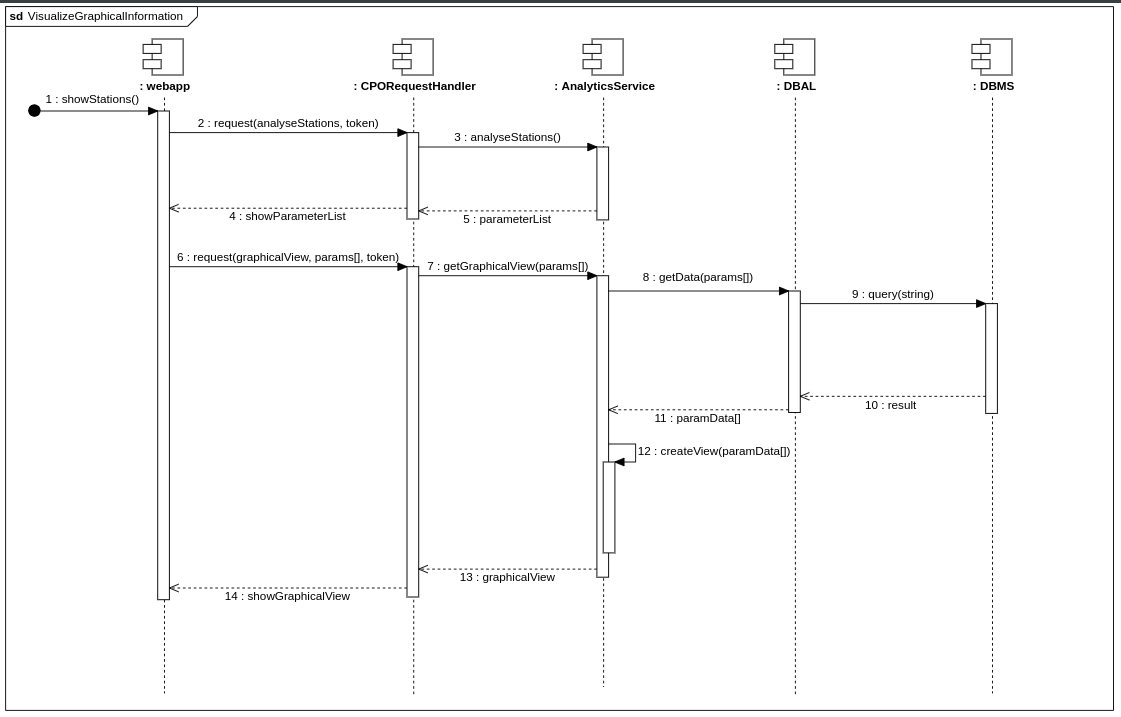
\includegraphics[trim={0 0cm 0 0.15cm},clip,width=1\textwidth]{Images/cp2/runtime/VisualizeGraphicalInformation.png}
    \caption{Visualize graphical information sequence diagram}
\end{figure}
The interaction starts when the CPO enters into the section available to analyse the stations. The web application returns a page with a list of parameters that the user can select in order to get a graphical view of the stations progress based on these criteria. Once selected the parameters the user confirms the operation, so he requests the graphical view based on his choices. The request is passed to the AnalyticsService component, which gets the needed data, depending on the desired analyses, and creates the graphical view using the acquired information. Then the graphical view is sent back to the web application, through the CPORequestHandler, and shown to the user.   

\clearpage
\textbf{StoreEnergyInBattery}\\
\begin{figure}[H]
    \centering
    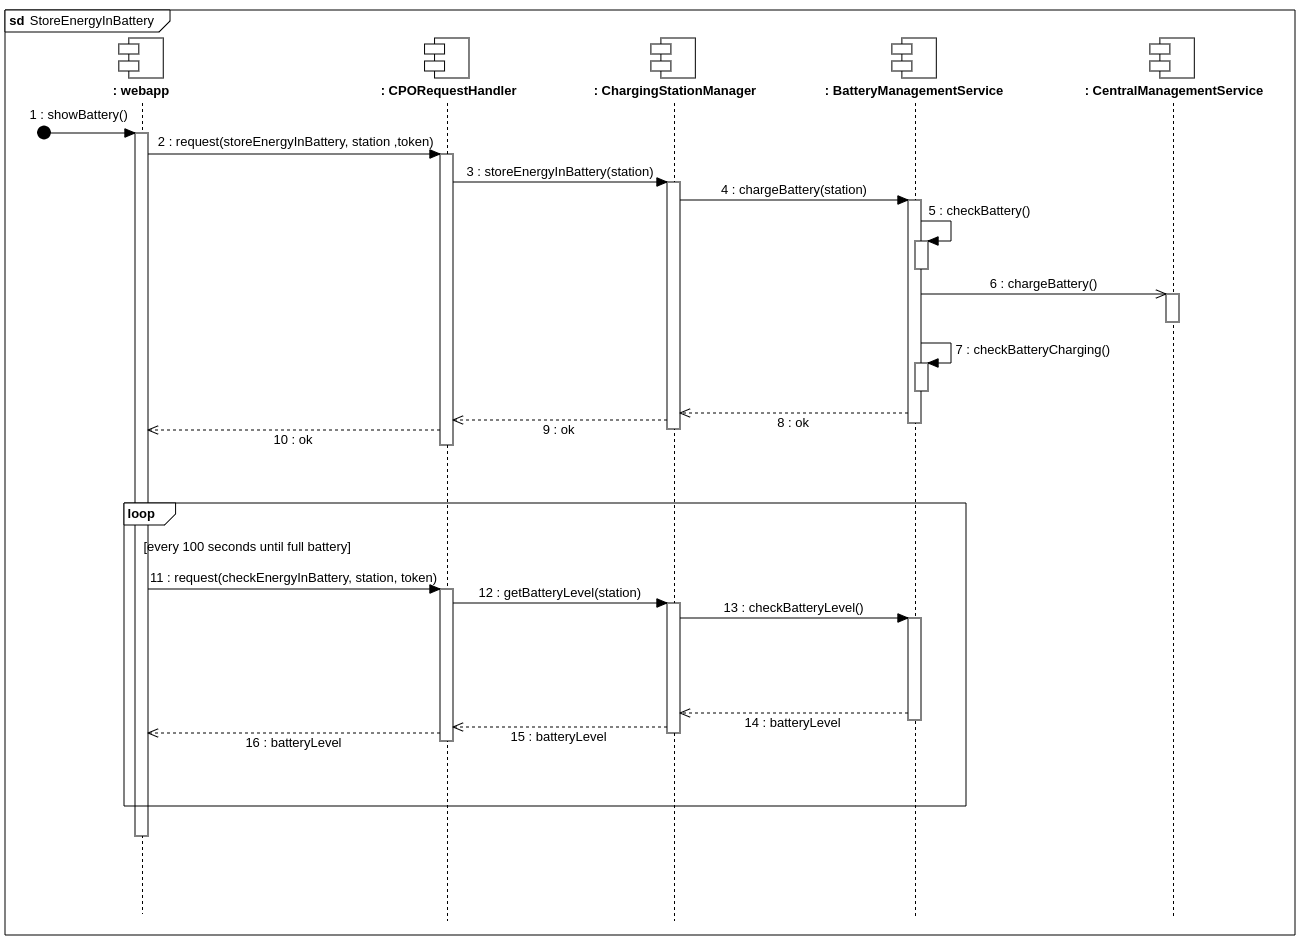
\includegraphics[width=1\textwidth]{Images/cp2/runtime/StoreEnergyInBattery.png}
    \caption{Charge battery sequence diagram}
\end{figure}
Once the CPO decides to store energy in the battery of a certain station that is equipped with it, the CPORequestHandler sends the request to the ChargingStationManager, which is the component that manages the changes of the stations, but it needs to interact with the BatteryManagementService, which checks the battery to see if it is full or can actually be charged and also checks if the battery is functional. If the battery can be charged an asynchronous message is sent to the CentralManagementService, that manages the technical aspects of the charging. The manager of the battery, then, controls if the battery is charging, and if the charging was correctly initiated the request is fulfilled. Finally, in loop, the web application interrogates the BatteryManagementService to know the level of the battery, keeping in this way track of the charging process and showing it to the user.  

\clearpage
\textbf{AddPromotion}\\
\begin{figure}[H]
    \centering
    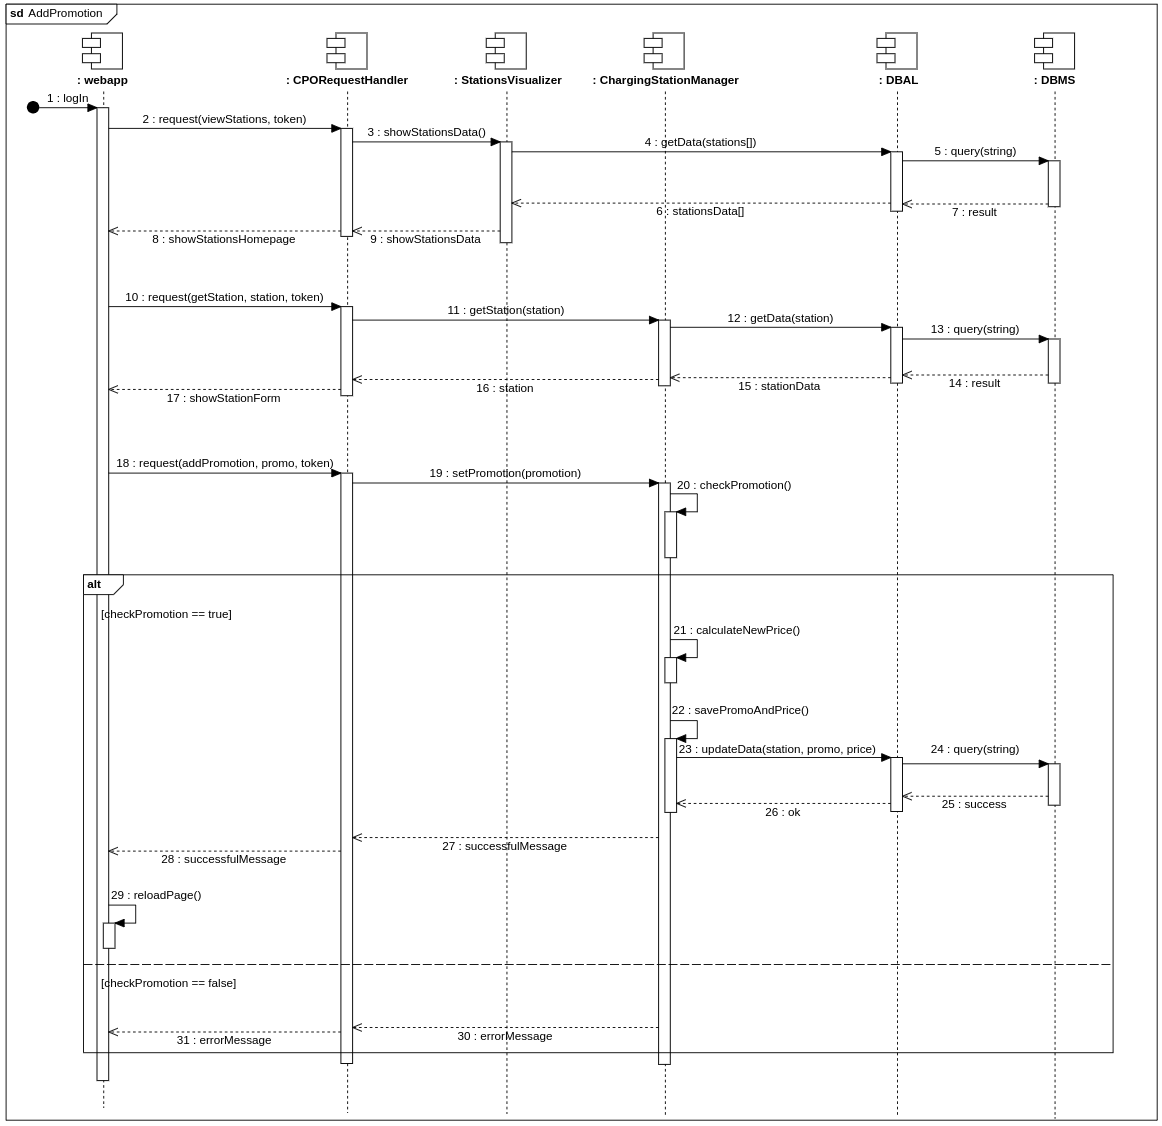
\includegraphics[width=1\textwidth]{Images/cp2/runtime/AddPromotion.png}
    \caption{Add promotion to charging station sequence diagram}
\end{figure}
To add a promotion to a charging station the CPO first selects the specific station, and then sets the promotion. The promotion is sent to the ChargingStationManager which checks the promotion, if it is compliant with the stations. If the promotion is acceptable the price is updated accordingly and the promotion and the price are saved on the DB. If the update is successful the page is reloaded. In this sequence diagram we see the main use case and the alternative one that treats the case of inserting an incorrect promotion, because we want to show how in case of error a lot of operations are not needed anymore.

\clearpage
\textbf{UpdateDSO}\\
\begin{figure}[H]
    \centering
    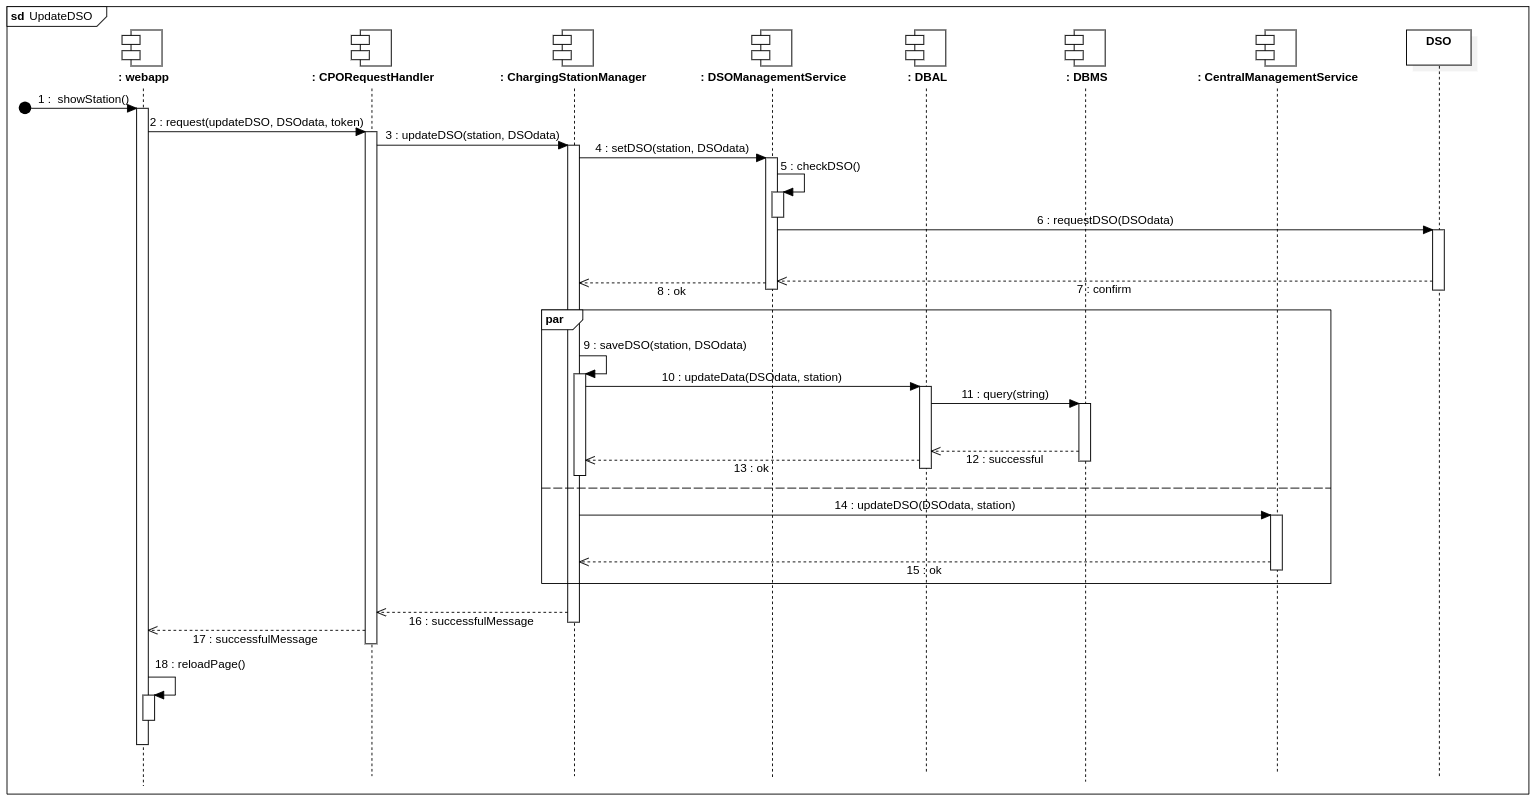
\includegraphics[width=1\textwidth]{Images/cp2/runtime/UpdateDSO.png}
    \caption{Update charging station DSO sequence diagram}
\end{figure}
Once selected a DSO and the relative data from the form, the station' DSO is updated. The ChargingStationManager sends to the DSOManagementService the station and the selected data of the DSO in order to check the data and send the request to the DSO itself. Once received a confirmation the DSOManagementService completes the update of the DSO and responds to the ChargingStationManager, which acknowledges the success. In parallel this component starts two operations, one that updates the data on the DB passing through the DBAL and DBMS, and another that updates the DSO data on the CentralManagementService. Once everything is updated the user receives a successful message and reloads the page. 

\clearpage
\section{Component interfaces}

\subsection{Common interfaces}
In this section we will list the interfaces of the components of out system. Since most of the functions and methods were already described in the previous section, we only give a description of the methods that might not result so straightforward to understand
\paragraph{DBAL}\mbox{}\\
\begin{table}[h]
    \centering
    \begin{tabular}{|l|}
        \hline
        \textbf{DBAL} \\
        \hline
        \verb|+ saveData(data): Boolean|\\
        \verb|+ getData(object): Object|\\
        \verb|+ getData(query): Object|\\
        \hline
    \end{tabular}
\end{table}
\\
The DBAL offers a layer of abstraction from the DBMS. It offers the ability to directly directly save objects with the method \verb|saveData|. Meanwhile for accessing it offers the capability to retrieve data from an object (like a map) or by making a query.

\paragraph{AuthenticationService}\mbox{}\\

\begin{table}[h]
    \centering
    \begin{tabular}{|l|}
        \hline
        \textbf{Authentication} \\
        \hline
         \verb|+ signup(email, password): Boolean|\\
         \verb|+ authenticate(email, password): Boolean|\\
         \verb|+ checkValidity(token): Boolean|\\
         \hline
    \end{tabular}
\end{table}
This component offers the classical interface for signing-up a user, likewise authenticate him and moreover provides the capability of validating the token possessed by the clients.

\paragraph{NotificationService}\mbox{}\\
\begin{table}[h]
    \centering
    \begin{tabular}{|l|}
        \hline
        \textbf{NotificationFormt} \\
        \hline
         \verb|+ notify(receiver, message)|\\
         \verb|+ sendEmail(email, content)|\\
         \hline
    \end{tabular}
\end{table}
\\
Notification Service offers the possibility to notify the client application of the user with the method \verb|notify(receiver, message)| and to send emails.

\subsection{eMSP interfaces}

\textbf{EVDRegistrationService}\\
\begin{table}[H]
    \centering
    \begin{tabular}{|l|}
        \hline
        \textbf{EVDRegistrationService} \\
        \hline
        \verb|+ register(name, surname, email): Boolean|\\
        \verb|+ setPassword(password): Boolean|\\
        \verb|+ registrationReady(): Boolean|\\
        \verb|- verifyUser()|\\
        \verb|+ sendLink(email)|\\
        \verb|+ saveUnverifiedUser(user)|\\
        \verb|+ sendRegistrationSuccess(email)|\\
        \hline
    \end{tabular}
\end{table}

\paragraph{PaymentService}\mbox{}\\
\begin{table}[H]
    \centering
    \begin{tabular}{|l|}
        \hline
        \textbf{PaymentService} \\
        \hline
         \verb|+ makePayment(paymentProcessor, credentials, amount): Boolean|\\
         \verb|+ savePayment(credentials, amount, timestamp): Boolean|\\
         \hline
    \end{tabular}
\end{table}
With the method \verb|makePayment| the PaymentService allows to user to perform a payment. Meanwhile the \verb|savePayment|, saves the payment instance on the DB. 
\paragraph{ChargingHistoryService}\mbox{}\\
\begin{table}[H]
    \centering
    \begin{tabular}{|l|}
        \hline
        \textbf{ChargingHistoryService} \\
        \hline
        \verb|+ getChargingHistory(user): ChargingSession[]|\\
        \verb|+ getChargingHistory(user, filter): ChargingSession[]|\\
        \verb|+ update(ChargingSession, updatedChargingSession): Boolean|\\
        \verb|+ delete(ChargingSession): Boolean|\\
        \hline
    \end{tabular}
\end{table}
\pagebreak
\textbf{EVDProfileManager}\\
\begin{table}[H]
    \centering
    \begin{tabular}{|l|}
        \hline
        \textbf{EVDProfileManager} \\
        \hline
        \verb|+ createProfile(name, surname, email, password)|\\
        \verb|+ updateUserDetails(user, field, newValue): Boolean|\\
        \verb|+ addEV(ev): Boolean|\\
        \verb|+ updateEV(user, ev, field, newValue): Boolean|\\
        \verb|+ deleteEV(user, ev): Boolean|\\
        \hline
    \end{tabular}
\end{table}

\textbf{ChargingSessionService}\\
\begin{table}[H]
    \centering
    \begin{tabular}{|l|}
        \hline
        \textbf{ChargingSessionService} \\
        \hline
        \verb|+ activateChargingPoint(chargingPointCode): Boolean|\\
        \verb|- openSession()|\\
        \verb|- closeSession()|\\
        \verb|- unlockChargingPoint()|\\
        \verb|+ changeStatus(chargingPoint, value)|\\
        \verb|+ addToOccupied(chargingPoint, user)|\\
        \verb|+ getStatus(chargingPoint): ChargingStatus|\\
        \hline
    \end{tabular}
\end{table}

\textbf{BookingService}\\
\begin{table}[H]
    \centering
    \begin{tabular}{|l|}
        \hline
        \textbf{BookingService} \\
        \hline
        \verb|+ bookChargingPoint(user, chargingPoint,|\\
        \hspace{4.2cm} \verb|startTimestamp, endTimestamp): Boolean|\\
        \verb|- openSession()|\\
        \verb|- closeSession()|\\
        \verb|- unlockChargingPoint()|\\
        \verb|+ makeReservation(chargingPoint, startTimestamp, endTimestamp): Boolean|\\
        \verb|+ cancelBooking(user, booking): Boolean|\\
        \verb|+ saveBooking(user, booking)|\\
        \hline
    \end{tabular}
\end{table}
\pagebreak
\textbf{ChargingStationDataManager}\\
\begin{table}[H]
    \centering
    \begin{tabular}{|l|}
        \hline
        \textbf{ChargingStationDataManager} \\
        \hline
        \verb|+ getStationsData(location, radius): Station[]|\\
        \verb|+ getStationFromChargingPoint(chargingPoint): Station|\\
        \verb|+ getStationsChargingPoints(station): ChargingPoint[]|\\
        \verb|+ collecDataFromCPMS(identifier)|\\
        \verb|+ updateDataFromCPMS(CPMS)|\\
        \verb|+ getStatus(chargingPoint): ChargingStatus|\\
        \verb|- openSession()|\\
        \verb|- closeSession()|\\
        \hline
    \end{tabular}
\end{table}
The method \verb|getStationsData(location, radius)| returns a collection of Station data structure containing all the information related to the charging stations that are are in the radius of the location provided as argument.\\
Moreover, the \verb|collectDataFromCPMS(identifier)| allows the system to collect the data of a new charging station managed by the CPMS identified by the identifier argument, which encodes the information to reach it. Meanwhile the method \verb|updateDataFromCPMS(CPMS)| updated the data of an already known CPMS.\\
\textbf{eMci}\\
\begin{table}[H]
    \centering
    \begin{tabular}{|l|}
        \hline
        \textbf{eMciControlAPI} \\
        \hline
        \verb|+ setCode(string)|\\
        \verb|+ getCode(): String|\\
        \hline
    \end{tabular}
\end{table}
The \verb|setCode(string)| allows to set the code that the user will use to start a charging session, while \verb|getCode()| can be used by the eMSP to know which code is set for that specific eMci.\\
\\
\textbf{EVDRequestHandler}\\
\begin{table}[H]
    \centering
    \begin{tabular}{|l|}
        \hline
        \textbf{EVDRequestHandler} \\
        \hline
        \verb|+ request(service, parameters[])|\\
        \verb|+ request(service, parameters[], token)|\\
        \hline
    \end{tabular}
\end{table}
The interface for the EVDRequestHandler is very simple, indeed it is composed of only two methods: one for the operations that do not require authorization and one for those that require it, as can be seen by the token required as argument. The signature tells us that to obtain the services of a component the requester shall indicate the service it want with the arguments to obtain it. This solution allows to implement the decouple the service offered from the component (or micro-service offering it), since will be the EVDRequestHandler to choose which component will respond to the request.\\

\textbf{eMma}\\
\begin{table}[H]
    \centering
    \begin{tabular}{|l|}
        \hline
        \textbf{Notification} \\
        \hline
        \verb|+ notifyUser(content)|\\
        \hline
    \end{tabular}
\end{table}
Interfaces implemented to allow the eMSP to notify the user in an asynchronous way.
\subsection{CPMS interfaces}
\textbf{ReservationService}\\
\begin{table}[H]
    \centering
    \begin{tabular}{|l|}
        \hline
        \textbf{ReservationService} \\
        \hline
        \verb|+ makeReservation(reservation): Boolean|\\
        \verb|+ checkAvailability(chargingPoint, startTimestamp, endTimestamp)|\\
        \verb|+ cancel(reservation): Boolean|\\
        \hline
    \end{tabular}
\end{table}

\textbf{ChargingStationInformationService}\\
\begin{table}[H]
    \centering
    \begin{tabular}{|l|}
        \hline
        \textbf{ChargingStationInformationService} \\
        \hline
        \verb|+ getChargingStationInfo(): JSONFile|\\
        \verb|+ getChargingPointsAvailability(): JSONFile|\\
        \hline
    \end{tabular}
\end{table}
This components through the method \verb|getChargingStationInfo()| returns a JSON file containing all the information regarding the charging station, including the charging points details. Meanwhile the \verb|getChargingPointsAvailability()| is used to query about the availability of the charging points. This method is included because we preview that this operation will happen more frequently and consequently this method is computationally less intensive and returns a lighter message.\\
\paragraph{eMSPRequestHandler}\mbox{}\\
\begin{table}[H]
    \centering
    \begin{tabular}{|l|}
        \hline
        \textbf{eMSPRequestHandler} \\
        \hline
        \verb|+ put(JSONObject[])|\\
        \verb|+ get(JSONObject[])|\\
        \verb|+ post(JSONObject[])|\\
        \verb|+ delete(JSONObject[])|\\
        \verb|+ patch(JSONObject[])|\\
        \hline
    \end{tabular}
\end{table}
This components implements the interface described for the OCPI protocol, here we only provide the list of methods this interface requires. For further information about the implementation of the OCPI protocol we reference the OCPI documentation\footnote{\url{www.evroaming.org/app/uploads/2021/11/OCPI-2.2.1.pdf}}.

\textbf{CentralManagementService}\\
\begin{table}[H]
    \centering
    \begin{tabular}{|l|}
        \hline
        \textbf{CentralManagementService} \\
        \hline
        \verb|+ unlockChargingPoint(chargeCode))|\\
        \verb|+ monitorChargingPoint(chargingPoint[])|\\
        \verb|+ chargeBattery()|\\
        \verb|+ disconnectBattery()|\\
        \verb|+ updateDSO(DSOData, station)|\\
        \hline
    \end{tabular}
\end{table}
\pagebreak
\textbf{DSOManagementService}\\
\begin{table}[H]
    \centering
    \begin{tabular}{|l|}
        \hline
        \textbf{DSOManagementService} \\
        \hline
        \verb|+ setDSO(station, DSODdata)|\\
        \verb|+ checkDSO()|\\
        \verb|+ addNewDSO(DSOdata)|\\
        \verb|+ refreshAllInfo()|\\
        \verb|+ refreshDSOInfo(DSO)|\\
        \verb|+ updateDSO(DSOData, station)|\\
        \hline
    \end{tabular}
\end{table}

\textbf{BatteryManagementService}\\
\begin{table}[H]
    \centering
    \begin{tabular}{|l|}
        \hline
        \textbf{BatteryManagementService} \\
        \hline
        \verb|+ chargeBattery(station)|\\
        \verb|+ stopChargingBattery(station)|\\
        \verb|+ getBatteryStatus(station): Status|\\
        \verb|+ getBatteryLevel(station): Percentage|\\
        \verb|+ setBatery(batteyCapacity)|\\
        \verb|- checkBattery()|\\
        \verb|- checkBatteryCharging(): Boolean|\\
        \hline
    \end{tabular}
\end{table}
The \verb|checkBattery()| is a private method used by the BatteryManagementService to check if the battery is functioning correctly (e.g. it's not broken). Meanwhile \verb|checkBatteryCharging()| check if the battery is charging.
\textbf{StationsVisualizer}\\
\begin{table}[H]
    \centering
    \begin{tabular}{|l|}
        \hline
        \textbf{StationsVisualizer} \\
        \hline
        \verb|+ showStationsData(): Stations[]|\\
        \verb|+ selectStation(id): Station|\\
        \hline
    \end{tabular}
\end{table}
The \verb|showStationsData()|, returns the collection of the stations managed by he CPO. By using the \verb|selectStation(id)| allows to get the Station from it's identifier.\\
\\
\clearpage
\textbf{AnalyticsService}\\
\begin{table}[H]
    \centering
    \begin{tabular}{|l|}
        \hline
        \textbf{AnalyticsService} \\
        \hline
        \verb|+ analyseStations(): Parameter[]|\\
        \verb|+ getGraphicalView(parameter[]): GraphicalView|\\
        \verb|+ createView(paramData[]): GraphicalView|\\
        \hline
    \end{tabular}
\end{table}

\textbf{ChargingStationManager}\\
\begin{table}[H]
    \centering
    \begin{tabular}{|l|}
        \hline
        \textbf{ChargingStationManager} \\
        \hline
        \verb|+ storeEnergyInBattery(station)|\\
        \verb|+ setPromotion(promotion)|\\
        \verb|+ setPrice(chargingPoint, price)|\\
        \verb|+ setPrice(station, price)|\\
        \verb|- calculateNewPrice()|\\
        \verb|- SavePromoAndPrice()|\\
        \verb|+ updateDSO(station, DSOdata)|\\
        \verb|+ getDSOdata(): DSO[]|\\
        \verb|+ addNewDso(DSOdata)|\\
        \verb|+ storeEnergyInBatttery(station)|\\
        \verb|+ stopBatteryCharging(station)|\\
        \verb|+ batteryStatus(station): Status|\\
        \verb|+ getBatteryLevel(station): BatteryLevel|\\
        \verb|+ setBattery(station, batteyCapacity)|\\
        \hline
    \end{tabular}
\end{table}
This is the component which interacts with the webapp and hides the internal implementation of the other components, hence many of its methods are not very simple, only calling homonymous methods of other components.\\

\textbf{DSORequestHandler}\\
\begin{table}[H]
    \centering
    \begin{tabular}{|l|}
        \hline
        \textbf{DSORequestHandler} \\
        \hline
        \verb|+ request(service, parameters[], token)|\\
        \hline
    \end{tabular}
\end{table}
The interface and behaviour of this component is identical to the EVDRequestHandler.\\
\textbf{webapp}\\
\begin{table}[H]
    \centering
    \begin{tabular}{|l|}
        \hline
        \textbf{Notification} \\
        \hline
        \verb|+ notifyUser(content)|\\
        \hline
    \end{tabular}
\end{table}

\pagebreak
\section{Selected architectural styles and patterns}
%3-layered architecture
\paragraph{A 3-layered Architecture}
The main architectural choice is to shape the application following the 3-layer architectural model, dividing the application into three main layers, as we can see in the deployment diagram.
The three main layers are: the presentation layer, the business logic layer, and the data access layer. Each layer has a specific role and communicates with the other layers through well-defined interfaces.

\begin{itemize}
    \item \textbf{Presentation layer}: This layer is responsible for handling the user interface and user interaction with the application. It includes the mobile app, the web app and the charging point interface
    \item \textbf{Business logic layer}: This layer is responsible for implementing the core functionality and business rules of the application. It includes all the micro-services with the respective code that handles all the functionalities to reach the goals of the system. These modules validate data, communicate with external systems and update the information of the charging stations and of the EVDs, in order to use the system on one hand to manage the stations and on the other hand to take advantage of the service itself, which is transparent and allows the booking and the charging of the EVs as main operations
    \item \textbf{Data access layer}: This layer is responsible for interacting with the database and providing data to the business logic layer as needed. It includes the DBMS, that handles tasks such as querying the database, inserting data, or updating records and this is an important tool to create, delete or update the database in a very fast and efficient way
\end{itemize}
\vspace{0.8cm}
There are several advantages in using a 3-layer architecture in an application with a mobile app for the users and a web app for the business managers:
\begin{itemize}
    \item \textbf{Separation of concerns and flexibility}: A 3-layer architecture helps to separate the different concerns of the application into different layers, which can make it easier to understand and maintain the codebase. For example, the presentation layer handles tasks related to rendering the UI and handling user input, while the business logic layer handles tasks related to calculating prices and validating data. This separation of concerns can make it easier to understand the different parts of the application and make changes to one part without affecting the others, so this gives more flexibility than a monolithic architecture
    \item \textbf{Modularity}: A 3-layer architecture also promotes modularity, which means that the different layers of the application can be developed and tested independently. This can make it easier to update and maintain the application, and allows to create better implementation and test plans
    \item \textbf{Scalability}: A 3-layer architecture can also be more scalable than a monolithic architecture, as it allows you to add or remove servers or resources as needed to handle an increase in traffic or load. This can be useful if the eMall experiences an increase in the number of users
\end{itemize}

\paragraph{MVC}
%MVC embedded in the choice of a 3-layer architecture
In the explained 3-layer architecture is embedded the MVC pattern:
\begin{itemize}
    \item \textbf{M - Model}: maps on the business layer and provides all the services to achieve the functionalities of the system and to access the database and acquire the necessary data to correctly provide information to the users 
    \item \textbf{V - View}: maps on the presentation layer and manages the interaction between the user and the system, and we have different views for the EVD and the CP
    \item \textbf{C - Controller}: receives the requests of the users and sends them to the interested services, so it is an intermediate component that hides the model from the view and communicates with both parts, creating a modularity of the system and allowing the separation of concerns and more flexibility as previously described in the 3-layered architecture
\end{itemize}
In the eMall we have as view the eMma, the eMci and the web app interface, which send the user requests to the specific controller, the eMSPRequestHandler and the CPORequestHandler respectively, that forward the request to the specific micro-services of the application layer. Also, from the application layer the components interact with the DBMS through the DBAL and acquire the data needed to process the request and respond to the user, sending the result back to the view passing through the controller.

\paragraph{Micro-services for the business layer}
%Micro-services in the business layer
Using the micro-services architecture for the business layer, the application is divided into a set of small, independently deployable services that communicate with each other. Each service is responsible for a specific function or business capability, and it is designed to be highly modular, scalable and resilient.\\
The eMma and the web app, through the interface of the presentation layer, communicate with the business logic layer via a set of micro-services, each of which is responsible for a specific service and interacts with the others to achieve the requirements of the system to be.\\
In the component diagrams we show these micro-services and the interaction between these modules. We separated them in the ones necessary for the eMSP server and the ones necessary for the CPMS server, underlying also the common services (as can be seen in the deployment diagram) that both parts of the system need to communicate with, such as the NotificationService, the AuthenticationService and the DBAL.\\\\
The micro-services architecture is well-suited to our system because being composed of independent services, if one fails, it will not bring down the entire system. This is perfect for our system because we want some services to be always running independently from the others. For example the CharginSessionService and BookingService are core services that should always be actively running and they do not depend from other secondary services like the EVDRegistrationService or the EVDProfileManager. The same can be said for the CPMS, the components granting access to the services of the charging stations to eMSPs should be independent from those that allow the CPO to manage the charging station, hence even if the CPO can't access the system to change some parameters, like updating the price, for the charging station, the EVDs can still book or start charging sessions. Furthermore, the system benefits from improved scalability. If the number of EVD increases we can increase the instances of the different handlers services (EVDRequestHandlers, eMSPRequestHanlder) to cope with the load increase, or alternatively, we could deploy these services in more powerful machines.

\section{Other design decisions}
\paragraph{Client-side rendering for the presentation layer}
Implementing the presentation layer with a client-side rendering approach, the web app and the mobile app on the client side are responsible for rendering the user interface.
In a client-side rendering architecture, the server typically responds to requests from the client by returning data that the client uses to dynamically generate the UI and this can be done using a front-end JavaScript framework such as React or Angular.
With client-side rendering, the initial page load is naturally a bit slow. However, after that, every subsequent page load is very fast, because there is no need to reload the entire UI after every call to the server. The client-side framework manages to update UI with changed data by re-rendering only some particular elements. This architecture can offer several benefits, such as better performance because the server doesn't have to generate the HTML on every request, and a better user experience, without requiring a full page reload.
We chose this approach mainly for the better user experience, having a more responsive application, and to manage a large number of clients without overloading the server. 

\paragraph{DBAL and DBMS to abstract the interaction with the databases}
%DBAL and DBMS
The DBAL is an application programming interface which unifies the communication between a computer application and databases. Database abstraction layers reduce the amount of work by providing a consistent API to the developer and hide the database specifics behind this interface as much as possible, so it allows to abstract from the technology adopted for the DB. This interface, then, passes the requests to the DBMS, which handles the main operations on the specific databases and provides several important functionalities\footnote{The DBMS information are retrieved from \url{https://www.javatpoint.com/functions-of-dbms}}:
\begin{itemize}
    \item Data Storage Management: creates a database for complex data and manages the data and allows the users to access it and manipulate the data very easily 
    \item Security Management and Multi User Access Control: provide a high level of security measures using various security algorithms to keep the data safe and ensure the data privacy, which is very import in our application which treats sensitive data of the EVDs, such as payment method and personal data, and also treats private business information for the management of the stations. There are certain security rules that ensure what data can be accessed from the database and which user can access it assuring security and privacy. So with the DBMS we can manage the different multi-user databases, shown in the deployment diagram: the EVDs database, the CPOs database and the shared database with the charging stations data. Also, more than one user can access the database at the same time without any problem, because the DBMS makes sure the integrity of the data present in the database is preserved and manages concurrency problems
    \item Backup and Recovery Management: to keep the data safe and ensure the integrity, the database system also provides the features for backup and recovery management, so if the system fails due to some reason then it recovers the most of the data 
    \item Database Access Language and Application Programming Interface and also Data Transformation and Presentation: provides the support of various query languages to access the databases and manipulate the data, so the three databases artifacts can use different data models and the DBMS allows to access them in the proper way without concerning the application with this interaction. This module also makes a data transformation, so the eMall programmers do not need to worry about the logical and physical representation of the data 
\end{itemize}

%What kind of database for the 3 artifacts

%Interaction with external APIs, do we have to say something about this? JEE framework?
